% ------------ begin cheatsheet
\documentclass[a4paper]{article}
\usepackage[a4paper,margin=0.05in]{geometry}
\usepackage{multicol}

\usepackage{varwidth}
\usepackage{xcolor}

\usepackage{amsmath, amssymb}
\usepackage[inline]{enumitem}
\usepackage{graphicx}

\usepackage{ulem}
\usepackage{makecell}

% horizontal list
\newlist{hlist}{enumerate*}{1}
\setlist[hlist]{label={}, afterlabel={}, itemjoin={{ \textbar{} }}}

% math
\newcommand{\abs}[1]{\left\lvert#1\right\rvert}

% envs
\newcommand{\oli}[1]{\begin{enumerate*}[label=(\arabic*)]#1\end{enumerate*}}

\graphicspath{ {./images/} }
\pagestyle{empty}
\setlength{\columnseprule}{0.3pt}

% reduce spacing before and after headers
\newcommand{\uppercaseandunderline}[1]{\uline{\uppercase{#1}}}

\makeatletter
\renewcommand{\section}{
  \@startsection{section}{1}{0pt}{1ex}{1.2ex} {\raggedleft\normalfont\large\bfseries\uppercaseandunderline}}
\renewcommand{\subsection}{
  \@startsection{subsection}{2}{0pt}{1ex}{1.2ex} {\raggedleft\normalfont\normalsize\bfseries\fbox}}
\renewcommand{\subsubsection}{
  \@startsection{subsubsection}{3}{0pt}{1ex}{0.8ex} {\raggedleft\normalfont\footnotesize\bfseries\uline}}
\renewcommand{\paragraph}{
  \@startsection{paragraph}{4}{0pt}{1.5ex}{-0.8em}{\normalfont\bfseries}}
% ------------ end cheatsheet

\newcommand{\red}[1]{\textcolor{red}{#1}}
\newcommand{\yellow}[1]{\colorbox{yellow}{#1}}

\begin{document}
\footnotesize
\setlength{\abovedisplayskip}{0pt}
\setlength{\belowdisplayskip}{0pt}
\setlength{\abovedisplayshortskip}{0pt}
\setlength{\belowdisplayshortskip}{0pt}
\begin{multicols*}{3}
  \part*{\centering \underline{CS3230}}
\section*{Asymptotic analysis}
  \subsection*{Word-RAM model}
    \begin{itemize}[leftmargin=*]
      \item Word is a collection of few bytes
      \item Word is the basic storage unit of RAM, which can be viewed as huge array of words
      \item Each input item is stored in binary format
      \item An arbitrary location of RAM can be accessed in the same time irrespective of the location
      \item Data and program fully reside in RAM
      \item Each arithmetic or logical operation involving a \textbf{constant number} of words takes \textbf{constant number of cycles (steps)} by the CPU
    \end{itemize}
  \subsection*{Big-O notation}
    \paragraph{Upper bound $(\geq)$} \mbox{} \\
      We write $f(n) = O(g(n))$ if for some $c > 0$ and $n_0 > 0$,
      \[ 0 \leq \textbf{f(n)} \leq c g(n) \]
      for all $n \geq n_0$.
    \paragraph{Lower bound $(\leq)$} \mbox{} \\ 
      We write $f(n) = \Omega(g(n))$ if for some $c > 0$ and $n_0 > 0$,
      \[ 0 \leq c g(n) \leq \textbf{f(n)} \]
      for all $n \geq n_0$.
    \paragraph{Tight bound} We write $f(n) = \Theta(g(n))$ if for some positive constants $c_1, c_2, n_0$,
      \[ 0 \leq c_1 g(n) \leq \textbf{f(n)} \leq c_2 g(n) \]
      for all $n \geq n_0$.
    \paragraph{Strict upper bound $(>)$} \mbox{} \\
      We write $f(n) = o(g(n))$ if for some $c > 0$ and $n_0 > 0$,
      \[ 0 \leq \textbf{f(n)} < c g(n) \]
      for all $n \geq n_0$.
    \paragraph{Strict lower bound $(<)$} \mbox{} \\ 
      We write $f(n) = \omega(g(n))$ if for some $c > 0$ and $n_0 > 0$,
      \[ 0 \leq c g(n) < \textbf{f(n)} \]
      for all $n \geq n_0$.
  \subsection*{Properties}
    \subsubsection*{Set notations}
      \begin{itemize}[leftmargin=*]
        \item The notations are really just sets, e.g.
          \begin{align*}
            O(g(n)) =\{& f(n): \exists c > 0, n_0 > 0 \text{ such that} \\
                       & 0 \leq f(n) \leq c(g(n)) \quad \forall n \geq n_0 \}
          \end{align*}
        \item $\Theta(g(n)) = O(g(n)) \cap \Omega(g(n))$
      \end{itemize}
    \subsubsection*{Transitivity} \noindent
      \begin{align*}
        f(n) = \Theta(g(n)) \land g(n) = \Theta(h(n)) & \Rightarrow f(n) = \Theta(h(n)) \\
        f(n) = O(g(n)) \land g(n) = O(h(n)) & \Rightarrow f(n) = O(h(n)) \\
        f(n) = \Omega(g(n)) \land g(n) = \Omega(h(n)) & \Rightarrow f(n) = \Omega(h(n)) \\
        f(n) = o(g(n)) \land g(n) = o(h(n)) & \Rightarrow f(n) = o(h(n)) \\
        f(n) = \omega(g(n)) \land g(n) = \omega(h(n)) & \Rightarrow f(n) = \omega(h(n))
      \end{align*}
    \subsubsection*{Reflexivity} \noindent
      \[
        f(n) = \Theta(f(n)) \quad
        f(n) = O(f(n)) \quad
        f(n) = \Omega(f(n))
      \]
    \subsubsection*{Symmetry} \noindent
      \[ f(n) = \Theta(g(n)) \iff g(n) = \Theta(f(n)) \]
    \subsubsection*{Complementarity} \noindent
      \begin{align*}
        f(n) = O(g(n)) &\iff g(n) = \Omega(f(n)) \\
        f(n) = o(g(n)) &\iff g(n) = \omega(f(n))
      \end{align*}
  \subsection*{Useful facts}
    \begin{itemize}[leftmargin=*]
      \item Degree-$k$ polynomials are $O(n^k)$, $o(n^{k+1})$, and $\omega(n^{k-1})$
      \item Polys dominate logs: \( (\log n)^{100} = o(n^{.0001}) \)
      \item Exponentials dominate polys: \( n^{1000} = o(2^{.001n}) \)
      \item $\max(f(n), g(n)) = \Theta(f(n) + g(n))$
    \end{itemize}
    \subsubsection*{Exponentials}
      \begin{itemize}[leftmargin=*]
        \item For constants $k>0, a>1, n^k = o(a^n)$
        \item Exponentials of different bases differ by an \textbf{exponential factor}
        \item $2^{n+5} = O(2^n)$, but $2^{5n} \neq O(2^n)$
      \end{itemize}
      \paragraph{Properties} \mbox{} \\
        \begin{minipage}{.475 \columnwidth}
          \begin{align*}
            a^{-1} &= \frac{1}{a} \\
            (a^m)^n &= a^{mn}
          \end{align*}
        \end{minipage}
        \begin{minipage}{.475 \columnwidth}
          \begin{align*}
            a^m a^n &= a^{m+n} \\
            e^x &\geq 1 + x
          \end{align*}
        \end{minipage}
    \subsubsection*{Logarithms} \noindent
      \begin{itemize}[leftmargin=*]
        \item Binary log: $\lg n = \log_2 n$
        \item Natural log: $\ln n = \log_e n$
        \item Exponentiation: $\lg^k n = (\lg n)^k$
        \item Composition: $\lg \lg n = \lg (\lg n)$
        \item Base of log does not matter in asymptotics:
          \[ \lg n = \Theta(\ln n) = \Theta(\log_{10} n) \]
      \end{itemize}
      \paragraph{Properties} \mbox{} \\
        \begin{minipage}{.475 \columnwidth}
          \begin{align*}
            a &= b^{\log_b a} \\
            \log_c(ab) &= \log_c a + \log_c b \\
            \log_b a^n &= n \log_b a \\
            \log_b a &= \frac{\log_c a}{\log_c b}
          \end{align*}
        \end{minipage}
        \begin{minipage}{.475 \columnwidth}
          \begin{align*}
            \log_b \frac{1}{a} &= - \log_b a \\
            \log_b a &= \frac{1}{\log_a b} \\
            a^{\log_b c} &= c^{\log_b a}
          \end{align*}
        \end{minipage}
    \subsubsection*{Overview} \noindent
      \begin{gather*}
        1 < \log n < \sqrt{n} < n < n \log n < n^2 \\
        < n^3 < 2^n < 2^{2n} < n! < n^n
      \end{gather*}
    \subsubsection*{Stirling's approximation} \noindent
      \begin{align*}
        n! &= \sqrt{2 \pi n} \left(\dfrac{n}{e}\right)^n \left(1 + \Theta\left(\frac{1}{n}\right)\right) \\
        \log(n!) &= \Theta(n \lg n)
      \end{align*}
    \subsubsection*{Arithmetic series} \noindent
      \[ \sum_{k=1}^n k = \frac{n(n+1)}{2} = \Theta(n^2) \]
    \subsubsection*{Geometric series} \noindent
      \begin{align*}
        \sum_{k=0}^n x^k &= \frac{x^{n+1} - 1}{x - 1} \\
        \sum_{k=0}^\infty x^k &= \frac{1}{1-x} \text{ when } \lvert x \rvert < 1
      \end{align*}
    \subsubsection*{Harmonic series} \noindent
      \[ \sum_{k=1}^\infty \frac{1}{k} = \ln n + O(1) \]
    \subsubsection*{Misc} \noindent
      \begin{gather*}
        \lg(\lg n)! = \Theta(\lg n \lg \lg n) \\
        \text{by subbing } \lg n \text{ into Stirling's approx.} \\
        \sum_{i=1}^{n-2} \lg \lg (n-i) = \Theta(n \lg \lg n) \\
        \sum_{i=1}^{\lg n-1} \lg \lg \frac{n}{2^i} = \Theta(\lg n \lg \lg n) \\
        n! > \left(\frac{n}{2}\right)^\frac{n}{2}
      \end{gather*}
      \begin{itemize}[leftmargin=*]
        \item For $T(n) = 2T(\sqrt{n}) + a$, the recursion tree has height $\lg \lg n$. Visualize by applying $\lg$ to each element of the recursion tree
        \item To compare two functions, consider taking the $\lg$ of each and compare that instead. This works since $\lg$ is strictly increasing
      \end{itemize}
  \subsection*{Limits} \noindent
    Assume $f(n), g(n) > 0$.
    \begin{align*}
      \lim_{n \rightarrow \infty} \frac{f(n)}{g(n)} = 0 &\Rightarrow f(n) = o(g(n)) \\
      \lim_{n \rightarrow \infty} \frac{f(n)}{g(n)} < \infty &\Rightarrow f(n) = O(g(n)) \\
      0 < \lim_{n \rightarrow \infty} \frac{f(n)}{g(n)} < \infty &\Rightarrow f(n) = \Theta(g(n)) \\
      \lim_{n \rightarrow \infty} \frac{f(n)}{g(n)} > 0 &\Rightarrow f(n) = \Omega(g(n)) \\
      \lim_{n \rightarrow \infty} \frac{f(n)}{g(n)} = \infty &\Rightarrow f(n) = \omega(g(n))
    \end{align*}
    \paragraph{Epsilon-delta definition}
      Let $f(x)$ be a function defined on an open interval around $x_0$, where $f(x_0)$ need not be defined. Then
      \[ \lim_{x \rightarrow x_0} f(x) = L \]
      if for every $\varepsilon$ there exists $\delta > 0$ such that for all $x$,
      \[ 0 < \lvert x - x_0 \rvert < \delta \implies \lvert f(x) - L \rvert < \varepsilon \]
    \paragraph{L'Hopital}
      If $\lim_{x \rightarrow \infty} f(x) = \lim_{x \rightarrow \infty} g(x) = 0 \text{ or } \pm \infty$,
      \[ \lim_{x \rightarrow \infty} \frac{f(x)}{g(x)} = \lim_{x \rightarrow \infty} \frac{f'(x)}{g'(x)} \]
    \paragraph{Power of $e$}
      \[ \lim_{n \rightarrow \infty} \left(1 + \frac{a}{n}\right)^{bn+c} = e^{ab} \]
  \subsection*{Recursive algorithms} \noindent
    Express time complexity in terms of recurrence:
    \[ T(n) = a T\left(\frac{n}{b}\right) + f(n) \]
    \subsubsection*{Master method} \noindent
      Comparing $f(n)$ with $n^{\log_b(a)}$ as polynomials, for $a \geq 1, b > 1, k \geq 0, \epsilon > 0$ and $f$ is asymptotically positive,
      \resizebox{\columnwidth}{!}{%
        \begin{math}
        \begin{aligned}
          & T(n) = a T\left( \frac{n}{b} \right) + f(n) & \\
          &= \begin{cases}
               \Theta(n^{\log_b(a)}) & f(n) = O(n^{\log_b(a) - \epsilon}) \\
               \Theta(n^{\log_b(a)} \log^{k+1} n) & f(n) = \Theta(n^{\log_b(a)} \log^k n) \\
               \Theta(f(n)) & f(n) = \Omega(n^{\log_b(a) + \epsilon})
             \end{cases}
        \end{aligned}
        \end{math}
      } \\
      For case 3, $f(n)$ must satisfy the regularity condition that $a f(n/b) \leq c f(n)$ for some $c < 1$, which guarantees that the sum of subproblems is smaller than $f(n)$. But this is typically satisified anyway.
    \subsubsection*{Substitution method}
      \begin{itemize}[leftmargin=*]
        \item Guess the form of the solution
        \item Verify by induction
      \end{itemize}
  \subsection*{Induction}
    \begin{itemize}[leftmargin=*]
      \item Verify base case
      \item Show that if the statement is true for the $k$th case (regular induction) or all cases up to the $k$th case (strong induction), then it is also true for the $(k+1)$th case
      \item Conclude that the statement is true for all cases
    \end{itemize}
\section*{Amortized analysis} \noindent
  Guarantees the average performance of each op in the worst case 
  \subsection*{Aggregate method}
    \begin{itemize}[leftmargin=*]
      \item Count total cost and divide by number of ops
    \end{itemize}
    \subsubsection*{Queues}
      \begin{itemize}[leftmargin=*]
        \item $n$ INSERT and EMPTY operations
        \item Notice EMPTY is a sequence of DELETES, and DELETES $\leq$ INSERTS
        \item If there are $k$ INSERTs, then sum of cost of all EMPTYs is $\leq k$
        \item Total cost $\leq k + k = 2k \leq 2n$ since $k \leq n$. Amortized cost is $O(1)$
      \end{itemize}
  \subsection*{Accounting method}
    \begin{itemize}[leftmargin=*]
      \item Charge $i$th operation a fictitious amoritzed cost $c(i)$, that satisfies
        \[ \sum_{i=1}^n t(i) \leq \sum_{i=1}^n c(i) \quad \forall n \]
        where $t(i)$ is the true cost of the $i$th operation
      \item Usually $c(i) > t(i)$, with the extra amount paid stored as credit for future, rare, expensive operations
      \item Analysis should ensure that there's always enough credit to pay for ture cost
      \item Always \textbf{identify the expensive operation}, which you try to do ``free of cost'' using stored credit
    \end{itemize}
    \subsubsection*{Queues}
      \begin{itemize}[leftmargin=*]
        \item For INSERT, set amortized cost to 2 (true cost is 1)
        \item For EMPTY, set amortized cost to 0 (true cost is size of queue)
        \item Whenever an element is inserted, we pay an extra 1. This extra 1 can be used as credit to pay for later deletions
        \item Total cost is at most $2 \; \times$ number of INSERTS $\leq 2n$
      \end{itemize}
    \subsubsection*{Binary increment}
      \begin{itemize}[leftmargin=*]
        \item Charge 2 for each $0 \rightarrow 1$; Charge 0 for each $1 \rightarrow 0$
        \item Starting from 0, actual cost for $n$ increments is $O(n)$
      \end{itemize}
  \subsection*{Potential method}
    \subsubsection*{Motivation}
      \begin{itemize}[leftmargin=*]
        \item Accounting method tries to eyepower the required amortized cost
        \item Potential method tries to find some metric that decreases a lot on expensive operations
        \item Similar idea
      \end{itemize}
    \subsubsection*{Idea}
      \begin{itemize}[leftmargin=*]
        \item Define potential function $\phi$, where $\phi(i)$ denotes potential at the end of the $i$th operation
        \item Must have $\phi(i) \geq 0$ for all $i$
        \item Amortized cost of $i$th op, $c(i)$ is defined as
          \yellow{
            $c(i) = t(i) + \Delta\phi$
          }
          where $\Delta \phi = \phi(i) - \phi(i-1)$
        \item Amortized cost of $n$th operations
          \[
            \sum_i c(i) = \sum_i t(i) + (\phi(n) - \phi(0)) \geq \sum_i t(i) - \phi(0)
          \]
        \item Select suitable $\phi$ so that for the \textbf{costly} operation, $\Delta \phi_i$ is \textbf{negative to an extent} that it nullifies or reduces the effect of the actual cost
      \end{itemize}
    \subsubsection*{Binary increment}
      \paragraph{Working}
        \begin{itemize}[leftmargin=*]
          \item Use $\phi(i) = $ number of 1s in the counter after $i$th increment
          \item Let $L_i$ be the length of the longest suffix with all 1s
          \item True cost of $i$th increment is $1 + L_i$
          \item $\Delta \phi_i = -L_i + 1$
          \item Sum of actual cost and $\Delta \phi_i$ is 2, so amortized cost of $i$th increment is 2
        \end{itemize}
      \paragraph{Results}
        \begin{itemize}[leftmargin=*]
          \item Starting from 0, actual cost for $n$ increments is $O(n)$
          \item Starting from $t$ ones, actual cost for $n$ increments is $O(n+t)$
        \end{itemize}
\section*{DP}
  \subsection*{\yellow{SRTBOT}}
    \begin{enumerate}[leftmargin=*]
      \item Subproblem definition
      \item Relate subproblem solutions recursively
      \item Topological order of subproblems to guarantee acyclic
      \item Base cases of relation
      \item Original problem: solve via subproblems
      \item Time analysis
    \end{enumerate}
  \subsection*{Examples shown} \noindent
    Fibonacci, LCS, Knapsack, Coin change
  \subsection*{Terminology}
    \subsubsection*{Optimal substructure} \noindent
      An optimal solution to a problem contains optimal solutions to subprobems
    \subsubsection*{Overlapping subproblems} \noindent
      A recursive solution contains a ``small'' number of distinct subproblems repeated many times
  \subsection*{\yellow{Cut-and-paste proof}} \noindent
    Often used to show optimal substructure
    \begin{enumerate}[leftmargin=*]
      \item Suppose your optimal solution is made using suboptimal solutions to subproblems
      \item Show that if you were to replace the suboptimal subproblem solutions with optimal subproblem solutions, you would improve your optimal solution
      \item Hence assumption is false, and the optimal solution is indeed made using optimal subproblem solutions
    \end{enumerate}
  \subsection*{
    \begin{varwidth}{\textwidth}
      Optimal substructure for \\ coin change
    \end{varwidth}
  } \noindent
    Let $M[j]$ denote the minimum number of coins required to change $j$ cents. Let the coins be $d_1, d_2, \cdots, d_k$.
    \\\\
    Suppose $M[j] = t$ is optimal, i.e.
    \[ j = d_{i_1} + d_{i_2} + \cdots + d_{i_t} \]
    for some $i_1, \cdots, i_t \in \{1, \cdots, k\}$.
    \begin{itemize}[leftmargin=*]
      \item Consider subproblem $j'$, where $j' = d_{i_1} + d_{i_2} + \cdots d_{i_{t-1}}$, and $M[j'] = t-1$
      \item If this were suboptimal, then $M[j'] < t-1$.
      \item By cut-and-paste argument, since we just need to add coin $d_{i_t}$ to subproblem $j'$ to reach subproblem $j$, then
        \[ M[j] = M[j'] + 1 < t-1 + 1 = t \]
      \item Contradicts the claim that $M[j] = t$ is optimal
      \item Hence the optimal solution is indeed made using optimal solutions to subproblems
    \end{itemize}
\section*{Greedy}
  \subsection*{Paradigm}
    \begin{enumerate}[leftmargin=*]
      \item Recast problem so that only one subproblem needs to be solved at each step
      \item Prove greedy-choice property
      \item Use optimal substructure to show that we can combine an optimal solution to the subproblem with the greedy choice, to get an optimal solution to the original problem
    \end{enumerate}
  \subsection*{Examples used} \noindent
    Fractional knapsack, Prim (MST), Choose top $k$ items
  \subsection*{Terminology} \noindent
    Refer to above for
    \begin{itemize}[leftmargin=*]
      \item Optimal substructure
      \item Overlapping subproblems
      \item Cut-and-paste proof
    \end{itemize}
    \subsubsection*{Greedy-choice property}
      \begin{itemize}[leftmargin=*]
        \item Locally optimal choice is also globally optimal
        \item Many optimal solutions may exist, but there is an optimal solution that made the greedy choice
      \end{itemize}
  \subsection*{Fractional knapsack}
    \subsubsection*{Optimal substructure} \noindent
      Let $x_i$ be the chosen weight for item $i$.
      \\\\
      Suppose $(x_1, \cdots, x_i \cdots, x_n)$ is an optimal solution to $\Big( (w_1, v_1), \cdots, (w_i, v_i), \cdots, (w_n, v_n), W \Big)$.
      \\\\
      WTS: $(x_1, \cdots, \red{x_i - w} \cdots, x_n)$ is an optimal soln to $\Big( (w_1, v_1), \cdots, \red{(w_i-w, v_i)}, \cdots, (w_n, v_n), \red{W} \Big)$.
      \begin{itemize}[leftmargin=*]
        \item Suppose \uline{better} solution for subproblem exists, i.e.
          \begin{itemize}[leftmargin=*]
            \item some $(y_1, \cdots, \red{y_i}, \cdots, y_n)$ weighs $\leq (W-w)$, with better value than $(x_1, \cdots, \red{x_i - w}, \cdots, x_n)$
          \end{itemize}
        \item Then $(y_1, \cdots, \red{y_i + w}, \cdots, y_n)$ weighs $\leq W$, and has better value than $(x_1, \cdots, \red{x_i}, \cdots, x_n)$
        \item Contradicts the claim that we had an optimal solution
        \item Hence the optimal solution is indeed made using optimal solutions to subproblems
      \end{itemize}
    \subsubsection*{Greedy choice property} \noindent
      Let $j^*$ be the item with the maximum value per kg, $v_j / w_j$.
      \\\\
      WTS: There exists an optimal knapsack containing $\min(w_{j^*}, W)$ kgs of item $j^*$, i.e. as much as possible of item $j^*$.
      \begin{itemize}[leftmargin=*]
        \item Suppose an \uline{optimal} knapsack contaings $x_1$ kgs of item 1, $x_2$ kgs of item 2, $\cdots$, $x_n$ kgs of item $n$, such that
          \[ x_1 + x_2 + \cdots + x_n = \min(w_{j^*}, W) \]
        \item We can replace this weight by $\min(w_{j^*}, W)$ kgs of item $j^*$
        \item Total weight does not change. Total value cannot decrease, because value per kg of $j^*$ is maximum. So knapsack stays optimal
      \end{itemize}
  \subsection*{MST}
    \subsubsection*{Definitions}
      \begin{itemize}[leftmargin=*]
        \item A graph $G = (V, E)$ is a pair consisting of
          \begin{itemize}[leftmargin=*]
            \item A set $V$ of vertices
            \item A set $E \subseteq V \times V$ of edges
          \end{itemize}
        \item $\lvert E \rvert = O(\lvert V \rvert^2)$
        \item Degree of a vertex $v$, $\mathrm{deg}(v)$ is the number of edges containing $v$
        \item Handshaking lemma: In any graph, $\sum_{v \in V} \mathrm{deg}(v) = 2 \cdot \lvert E \rvert$
      \end{itemize}
    \subsubsection*{Spanning tree}
      \begin{itemize}[leftmargin=*]
        \item A graph is connected if there is a path between any two vertices
        \item A tree is a connected graph without cycles
        \item A spanning tree of a connected graph $G = (V, E)$ is a tree that contains all of the vertices from $V$, and a subset of edges from $E$
        \item Given a weight function $w: E \rightarrow \mathbb{R}$, the weight of a spanning tree $T$ is
          \[ \sum_{(u,v) \in T} w(u,v) \]
        \item A minimum spanning tree is a spanning tree with minimum weight
      \end{itemize}
    \subsubsection*{Optimal substructure} \noindent
      Any sub-tree $T_k$ of the MST $T$ is an MST of the subgraph induced by the vertices of $T_k$
    \subsubsection*{Greedy-choice property} \noindent
      The least weight edge connecting any set of vertices to its complement is contained in the MST
\section*{Max flow}
  \subsection*{Terminology}
    \subsubsection*{Flow network}
      \begin{itemize}[leftmargin=*]
        \item A flow network is a directed graph $G = (V,E)$ in which
          \begin{itemize}[leftmargin=*]
            \item If $(u,v) \in E$, then capacity $c(u,v) \geq 0$
            \item If $(u,v) \not\in E$, then capacity $c(u,v) = 0$
          \end{itemize}
        \item For simplicity, no self-loops, no anti-parallel edges ($A \rightarrow B \rightarrow A$)
      \end{itemize}
    \subsubsection*{Flow} \noindent
      A flow is a function $f$ that assigns a number $f(u,v)$ to each edge - the flow from $u$ to $v$. It satisfies two properties:
      \begin{enumerate}[leftmargin=*]
        \item Capacity: Flow $\leq$ Capacity
          \[ \forall (u,v) \in E, \quad 0 \leq f(u,v) \leq c(u,v) \]
        \item Flow conservation: Flow in = Flow out
          \[ \sum_{v \in V} f(v, u) = \sum_{v \in V} f(u, v) \]
      \end{enumerate}
    \subsubsection*{Max flow} \noindent
      \begin{itemize}[leftmargin=*]
        \item The value of a flow $f$ is
          \[ \lvert f \rvert = \sum_{v \in V} f(s,v) \]
          assuming $s$ has no incoming edges
        \item Max flow maximizes the value $\lvert f \rvert$ for a flow from start node $s$ to destination node $t$
      \end{itemize}
  \subsection*{Bipartite matching} \noindent
    \subsubsection*{Problem}
      \begin{itemize}[leftmargin=*]
        \item Matching: A subset of edges such that each vertex is part of at most one edge
        \item Given a bipartite graph, what is the largest number of edges a matching can have
      \end{itemize}
    \subsubsection*{Solution} \noindent
      Bipartite matching reduces to max flow.
      \begin{itemize}[leftmargin=*]
        \item Connect node $s$ to all nodes in left half
        \item Connect all nodes in right half to node $t$
        \item Set all edges to have capacity 1
      \end{itemize}
      Need to show that the flow at each edge is either 1 or 0, to correspond to a bipartite matching solution. Running Ford-Fulkerson should guarantee this
  \subsection*{Ford-Fulkerson}
    \subsubsection*{Formal algorithm}
      \begin{enumerate}[leftmargin=*]
        \item Start $f(u,v) = 0$ for all $u, v$
        \item While there is a path $p$ from $s$ to $t$ in $G_f$,
          \begin{itemize}[leftmargin=*]
            \item Let $m = \min_{(u,v) \in p} c_f (u,v)$
            \item For each $(u,v) \in p$,
              \begin{itemize}[leftmargin=*]
                \item If $(u,v) \in E$, increment $f(u,v)$ by $m$
                \item If $(v,u) \in E$, decrement $f(v,u)$ by $m$
              \end{itemize}
          \end{itemize}
      \end{enumerate}
    \subsubsection*{Residual capacities} \noindent
      Given a flow $f$, define residual capacities $c_f$, which represents the remaining capacities:
      \begin{itemize}[leftmargin=*]
        \item If $(u,v) \in E$, $c_f(u,v) = c(u,v) - f(u,v)$
        \item If $(v,u) \in E$, $c_f(u,v) = f(v,u)$
        \item Else, $c_f(u,v) = 0$
      \end{itemize}
    \subsubsection*{Residual graph}
      \begin{itemize}[leftmargin=*]
        \item Residual graph $G_f$ keeps track of the capacities in ``each direction''
        \item For example, if the path $s \rightarrow a \rightarrow c \rightarrow b \rightarrow d \rightarrow t$ is chosen, we can push a flow of 4 and get the following residual graph
      \end{itemize}
      \begin{center}
        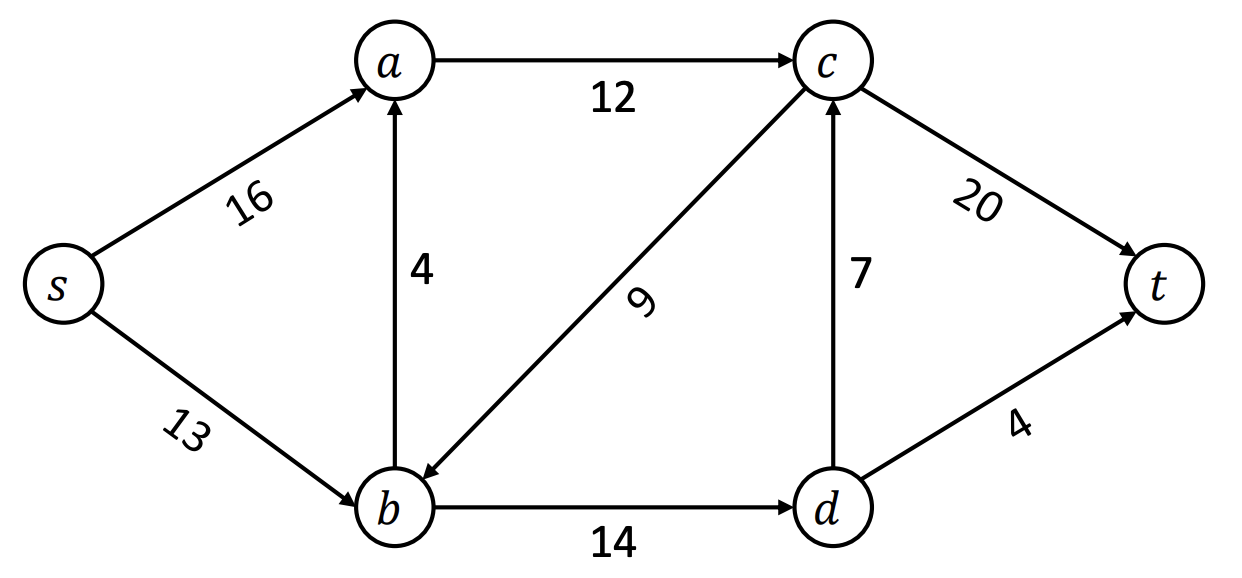
\includegraphics[width=\columnwidth]{L9/original}
        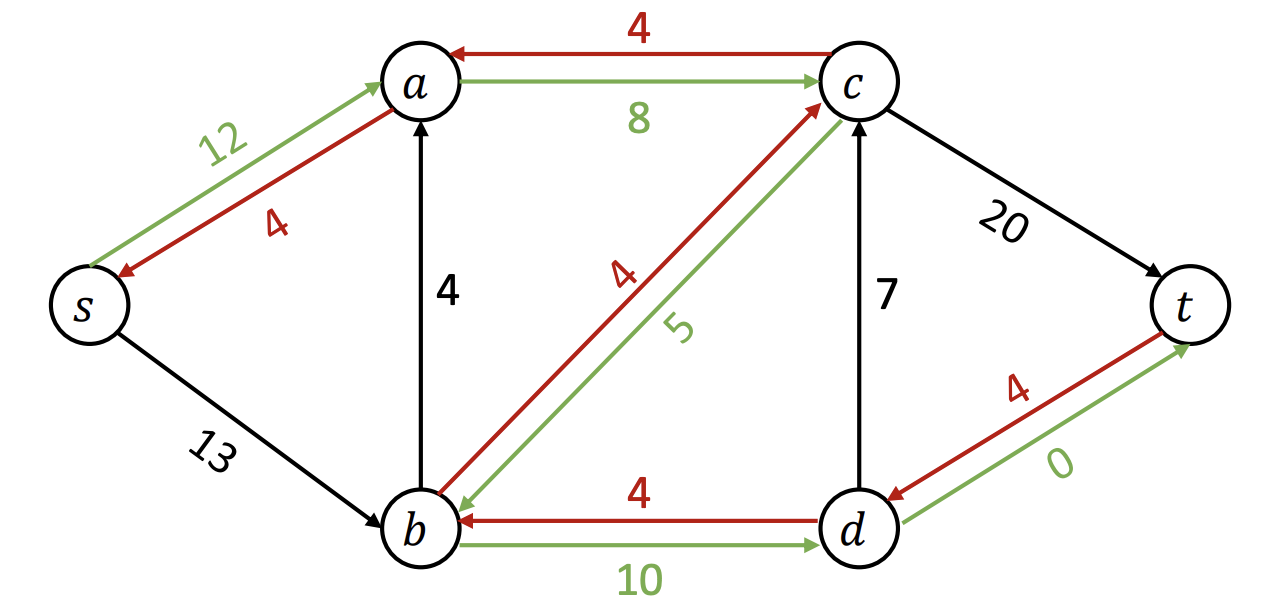
\includegraphics[width=\columnwidth]{L9/residual}
      \end{center}
    \subsubsection*{Instantiation} \noindent
      Ford-Fulkerson does not specify how the path should be found
      \begin{itemize}[leftmargin=*]
        \item Find using DFS: $O(\lvert E \rvert \cdot \lvert f_{max} \rvert)$, where $f_{max}$ is the maximal flow
        \item Edmonds-Karp algorithm - find (unweighted) shortest path using BFS: $O( \lvert V \rvert \lvert E \rvert^2 )$:
      \end{itemize}
  \subsection*{Max flow vs min cut}
    \begin{center}
      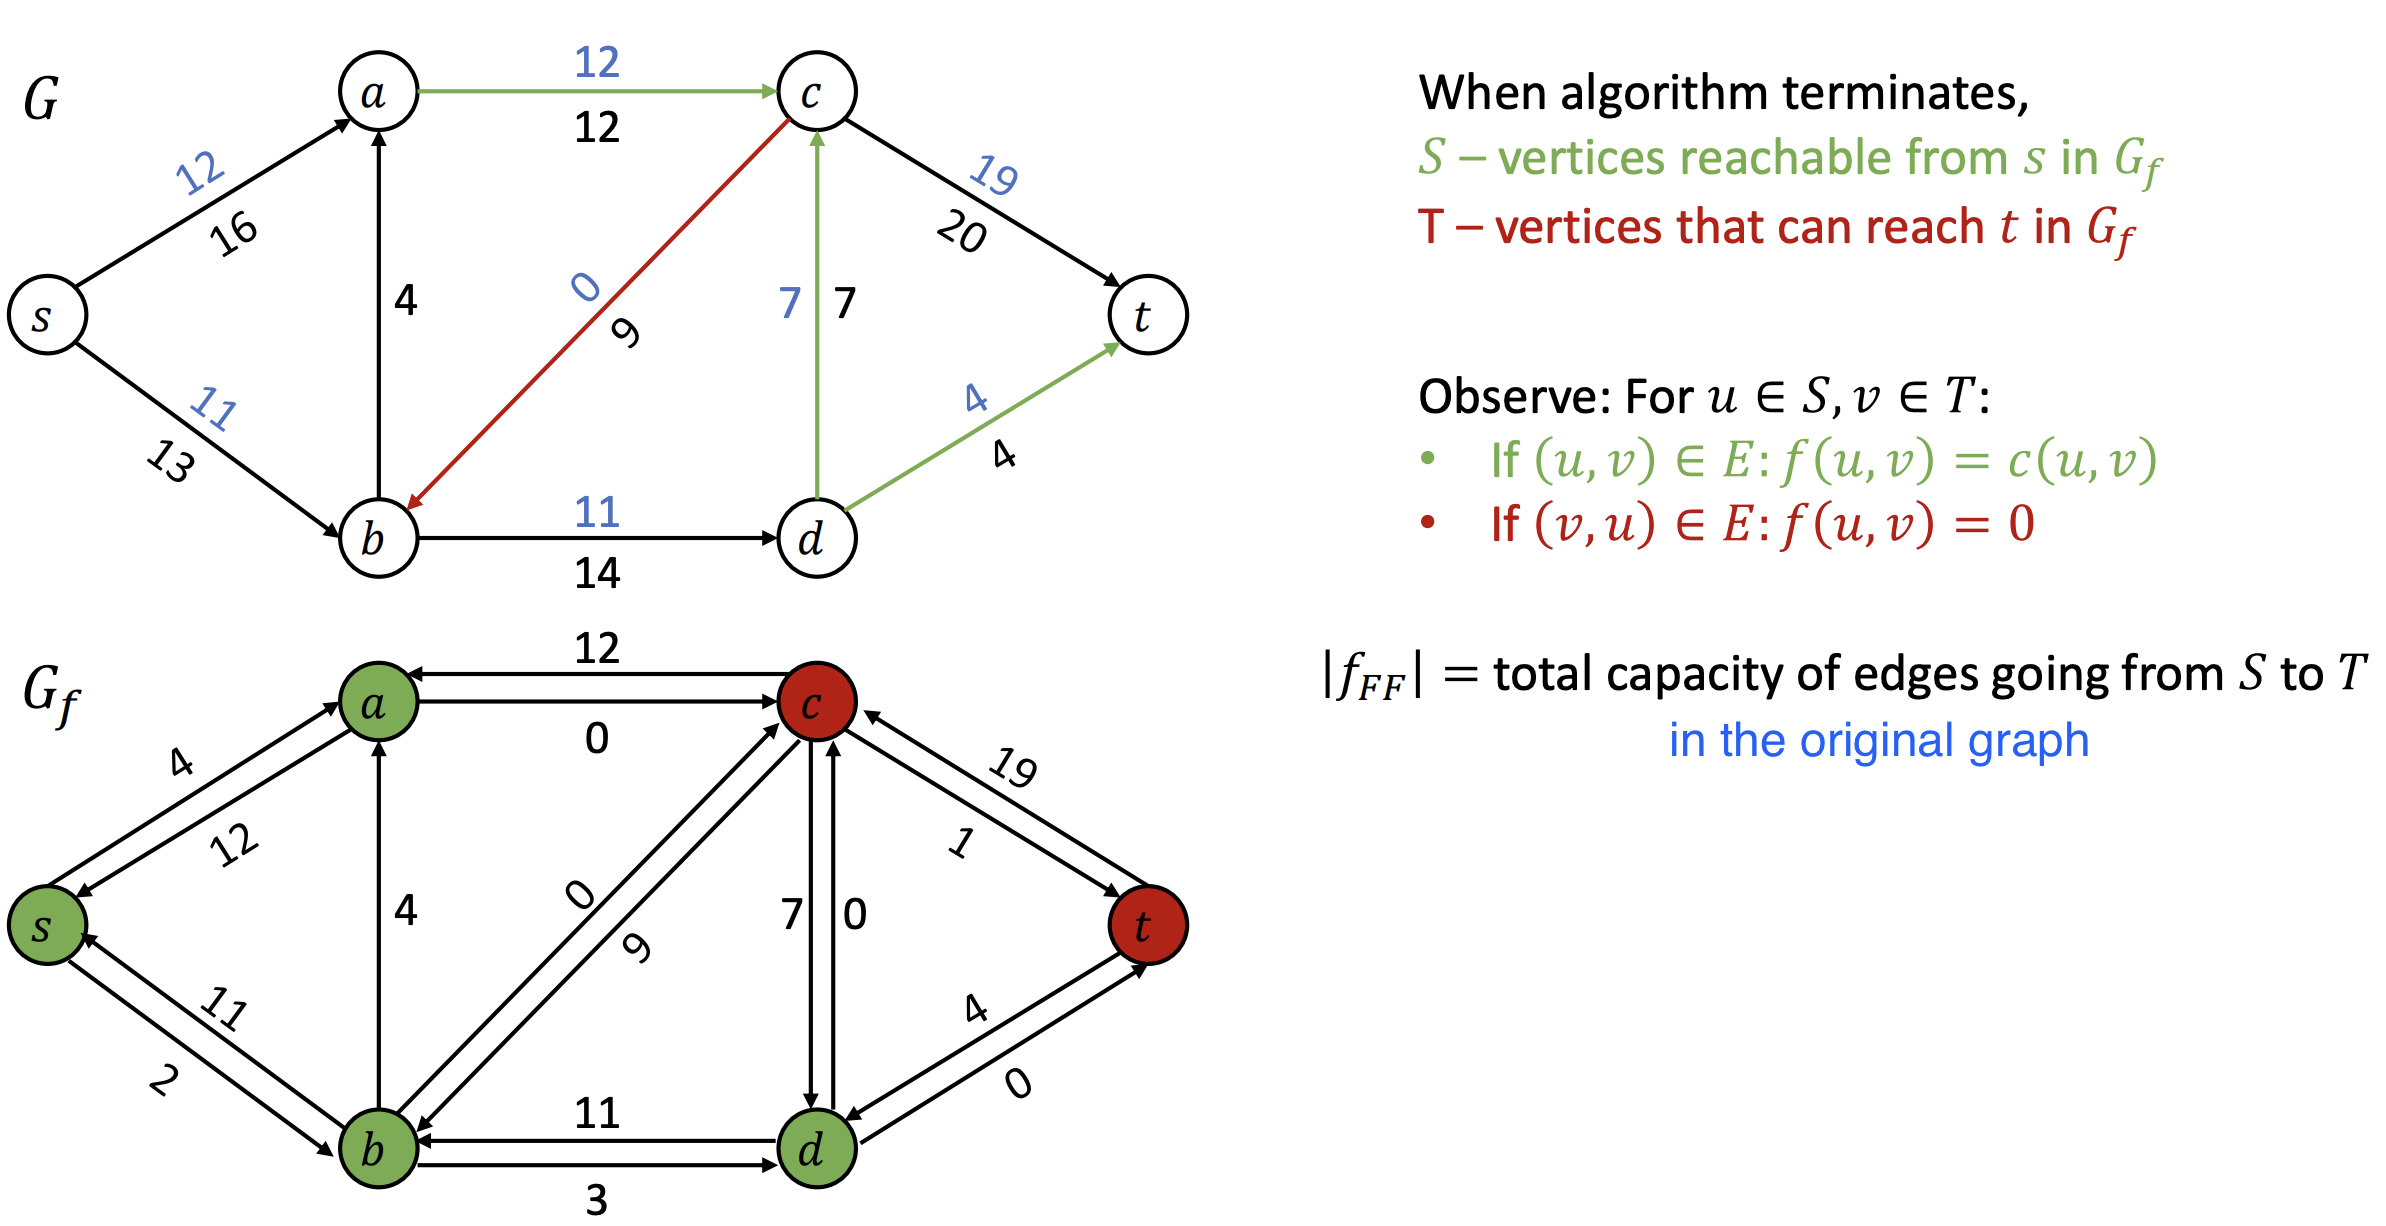
\includegraphics[width=\columnwidth]{L9/min_cut_1}
      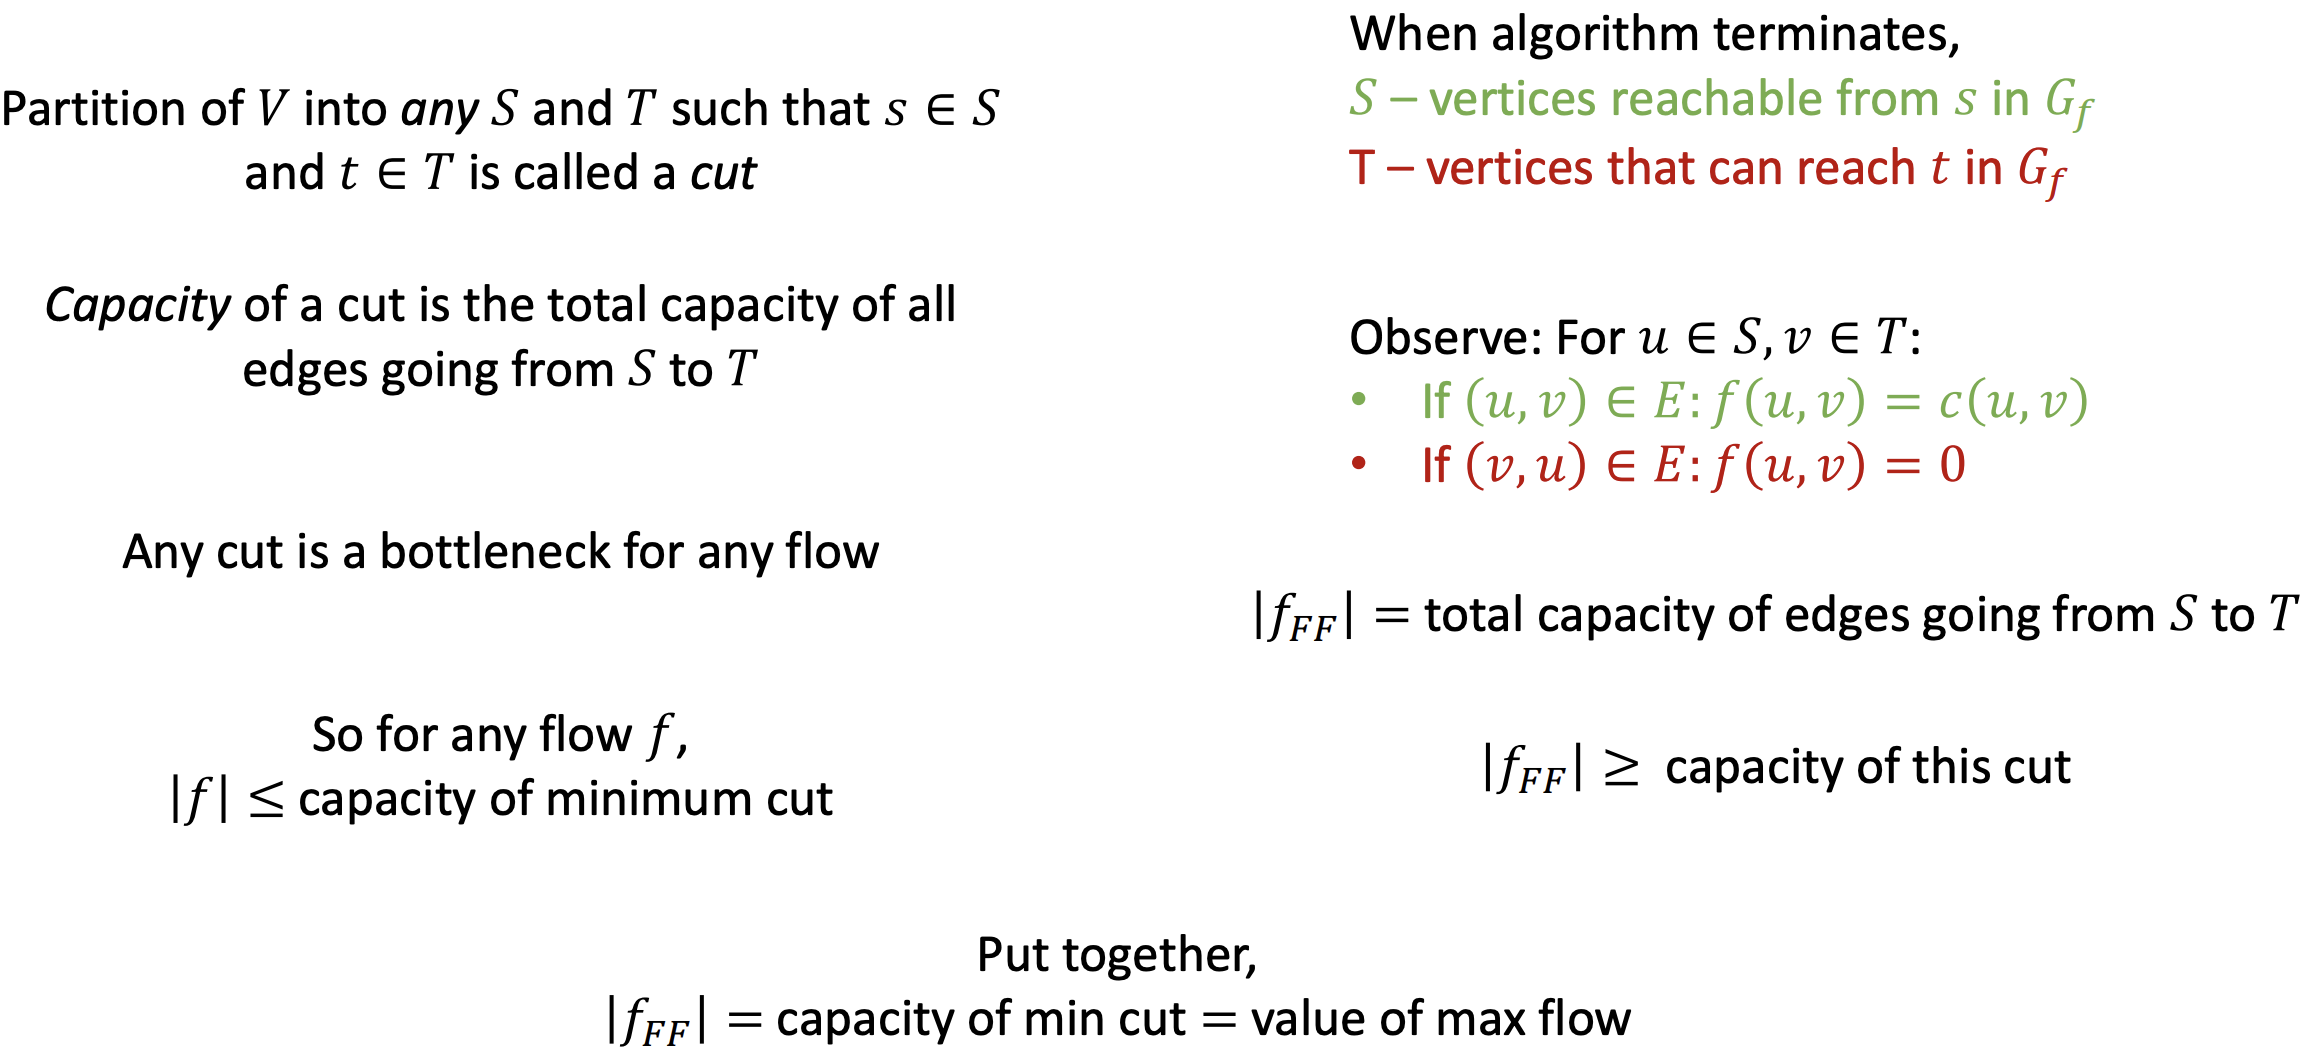
\includegraphics[width=\columnwidth]{L9/min_cut_2}
    \end{center}
\section*{Linear Programming}
  \subsection*{Definition}
    \begin{itemize}[leftmargin=*]
      \item Variables $x_1, \cdots, x_n$
      \item Maximize linear sum $\sum_{j \in [n]} c_j \cdot x_j$
      \item Subject to constraints which are linear inequalities:
    \end{itemize}
    \begin{gather*}
      x_1, \cdots, x_n \geq 0 \\
      a_{11}x_1 + \cdots + a_{1n}x_n \leq b_1 \\
      a_{21}x_1 + \cdots + a_{2n}x_n \leq b_2 \\
      \cdots \\
      a_{m1}x_1 + \cdots + a_{mn}x_n \leq b_m
    \end{gather*}
    \begin{itemize}[leftmargin=*]
      \item Any LP can be converted into this standard form
      \item Optimal solution (if exists) can be found in $poly(n, m)$ time
    \end{itemize}
  \subsection*{\yellow{Converting to standard form}}
    \subsubsection*{Minimize instead of maximize objective} \noindent
      Minimize $f(x) \implies$ Maximize $-f(x)$
    \subsubsection*{Unbounded variables} \noindent
      If $x_1 \in \mathbb{R}$, then $x_1 = x_2 - x_3$, where $x_2, x_3 \geq 0$
    \subsubsection*{Equality constraints} \noindent
      If $a x_1 + b x_2 = c$, then we can express this as two constraints:
      \begin{align*}
        -a x_1 + -b x_2 &\leq -c \\
        a x_1 + b x_2 &\leq c
      \end{align*}
    \subsubsection*{Sum of absolute values} \noindent
      Use linear programming to find a solution $(a,b)$ that minimizes
      \[ \sum_{i=1}^n \lvert y_i - ax_i - b \rvert \]
      Define $e_i = \lvert y_i - ax_i - b \rvert$ such that
      \begin{itemize}[leftmargin=*]
        \item $y_i - ax_i - b \leq e_i$
        \item $y_i - ax_i - b \geq -e_i$
        \item $e_i \geq 0$
      \end{itemize}
    \subsubsection*{Minimizing a max function} \noindent
      For minimizing $z = \max x_i$, define constraints $z \geq x_i$
  \subsection*{Visualizing}
    \begin{center}
      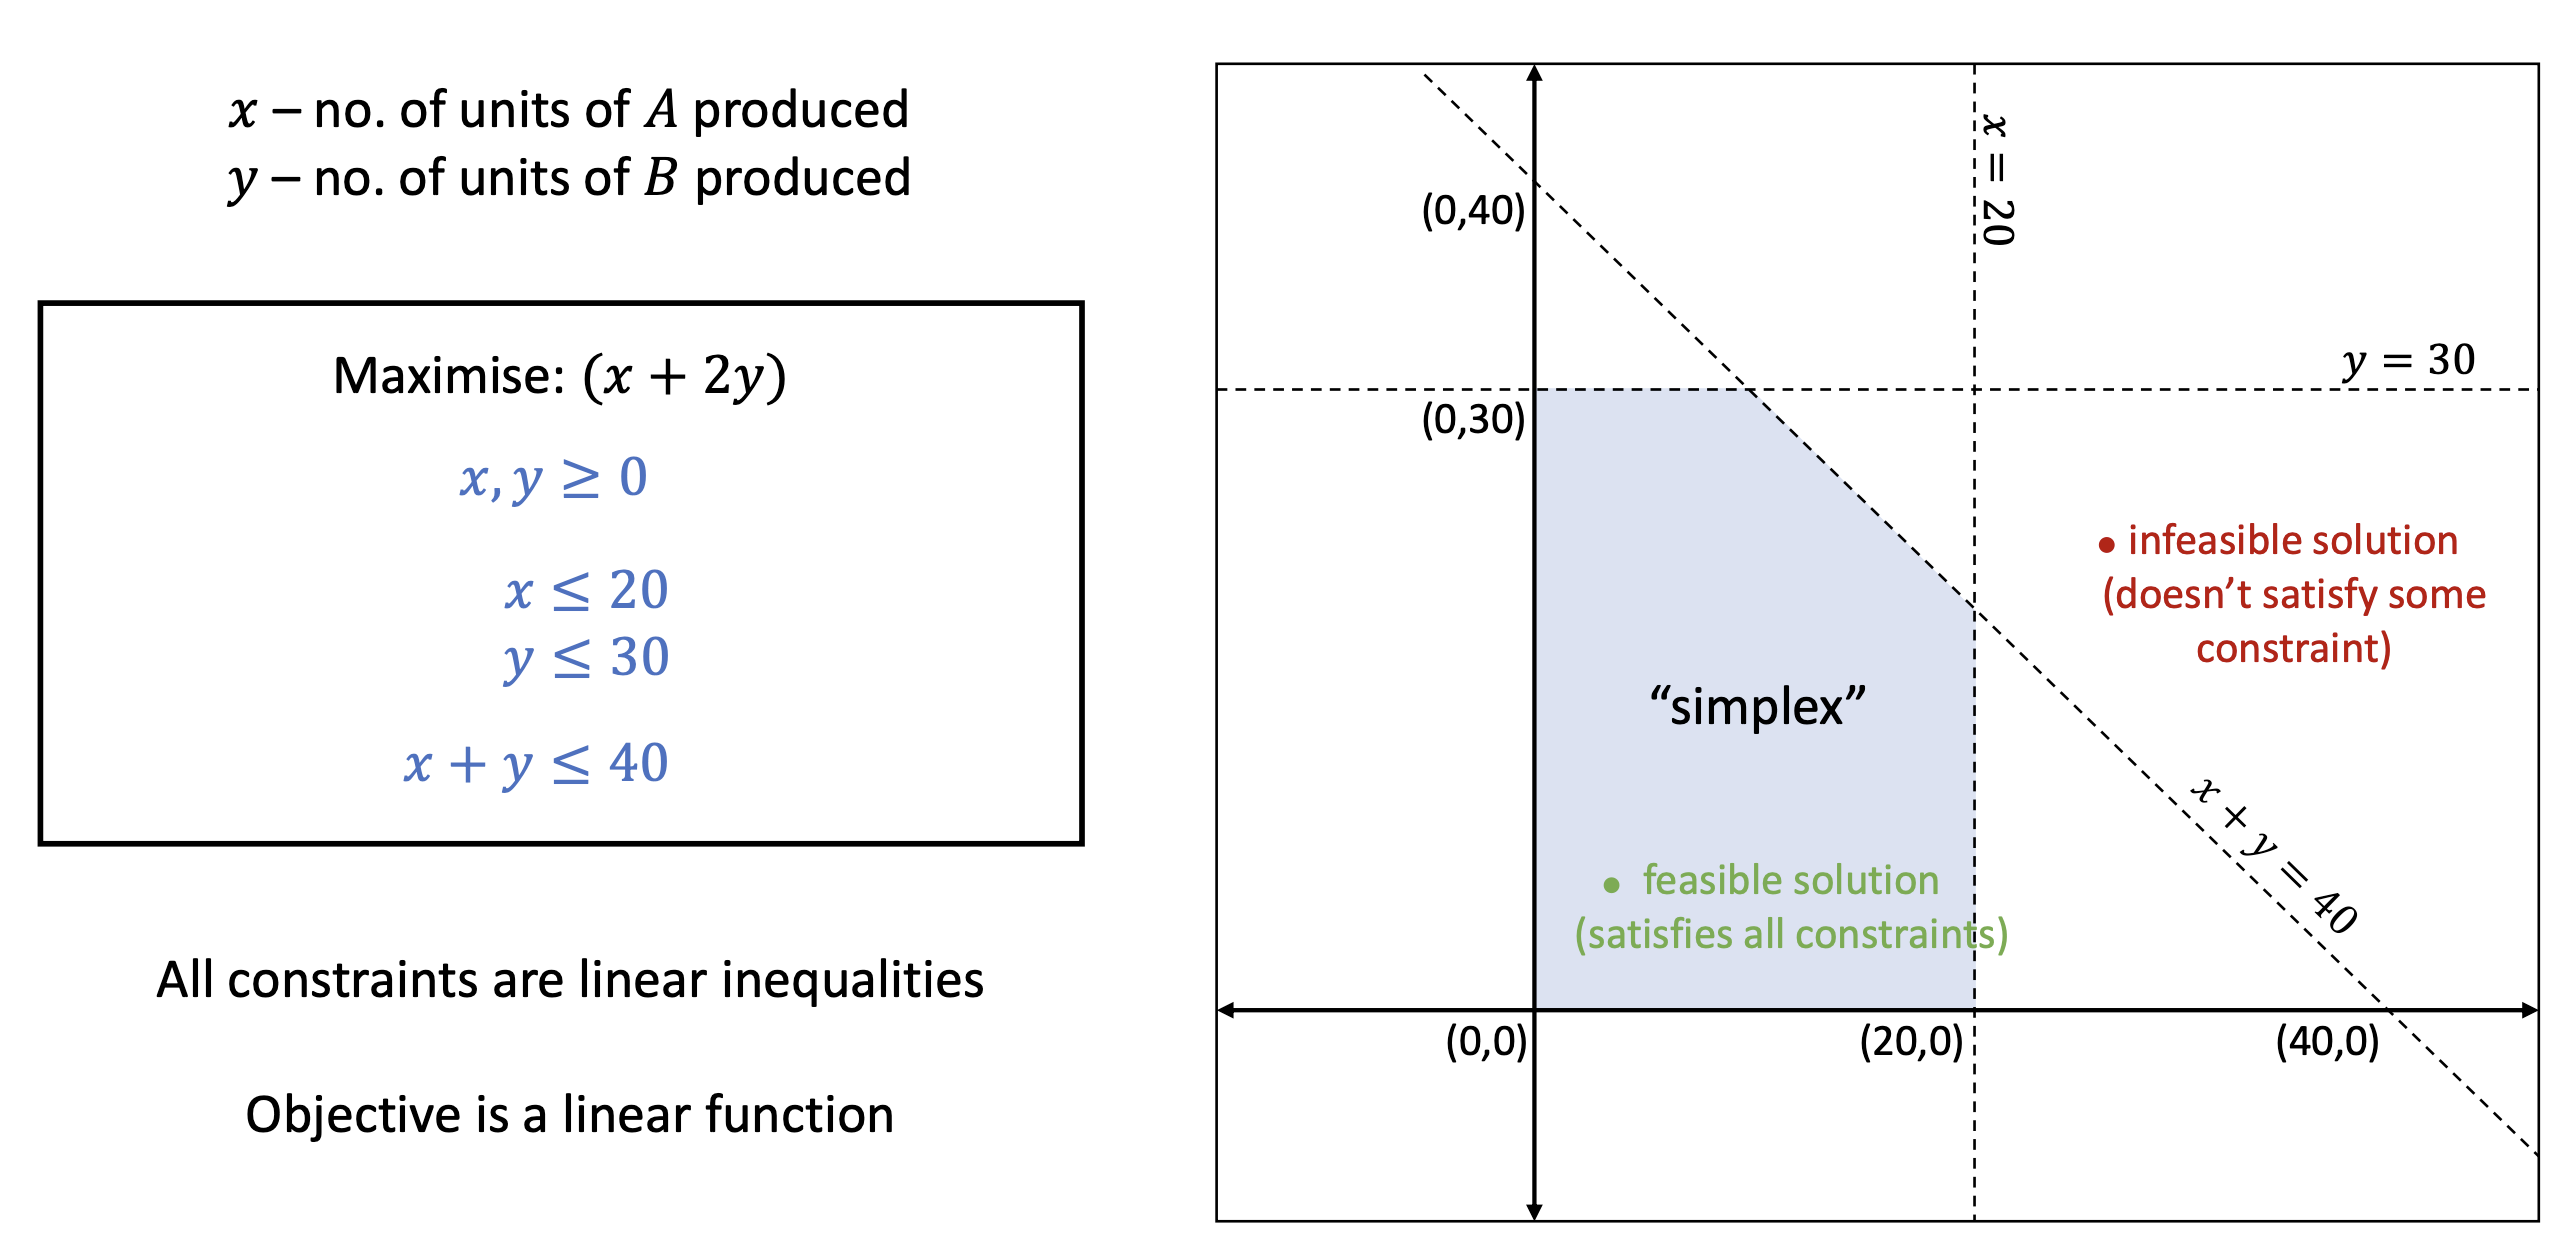
\includegraphics[width=\columnwidth]{L10/simplex}
      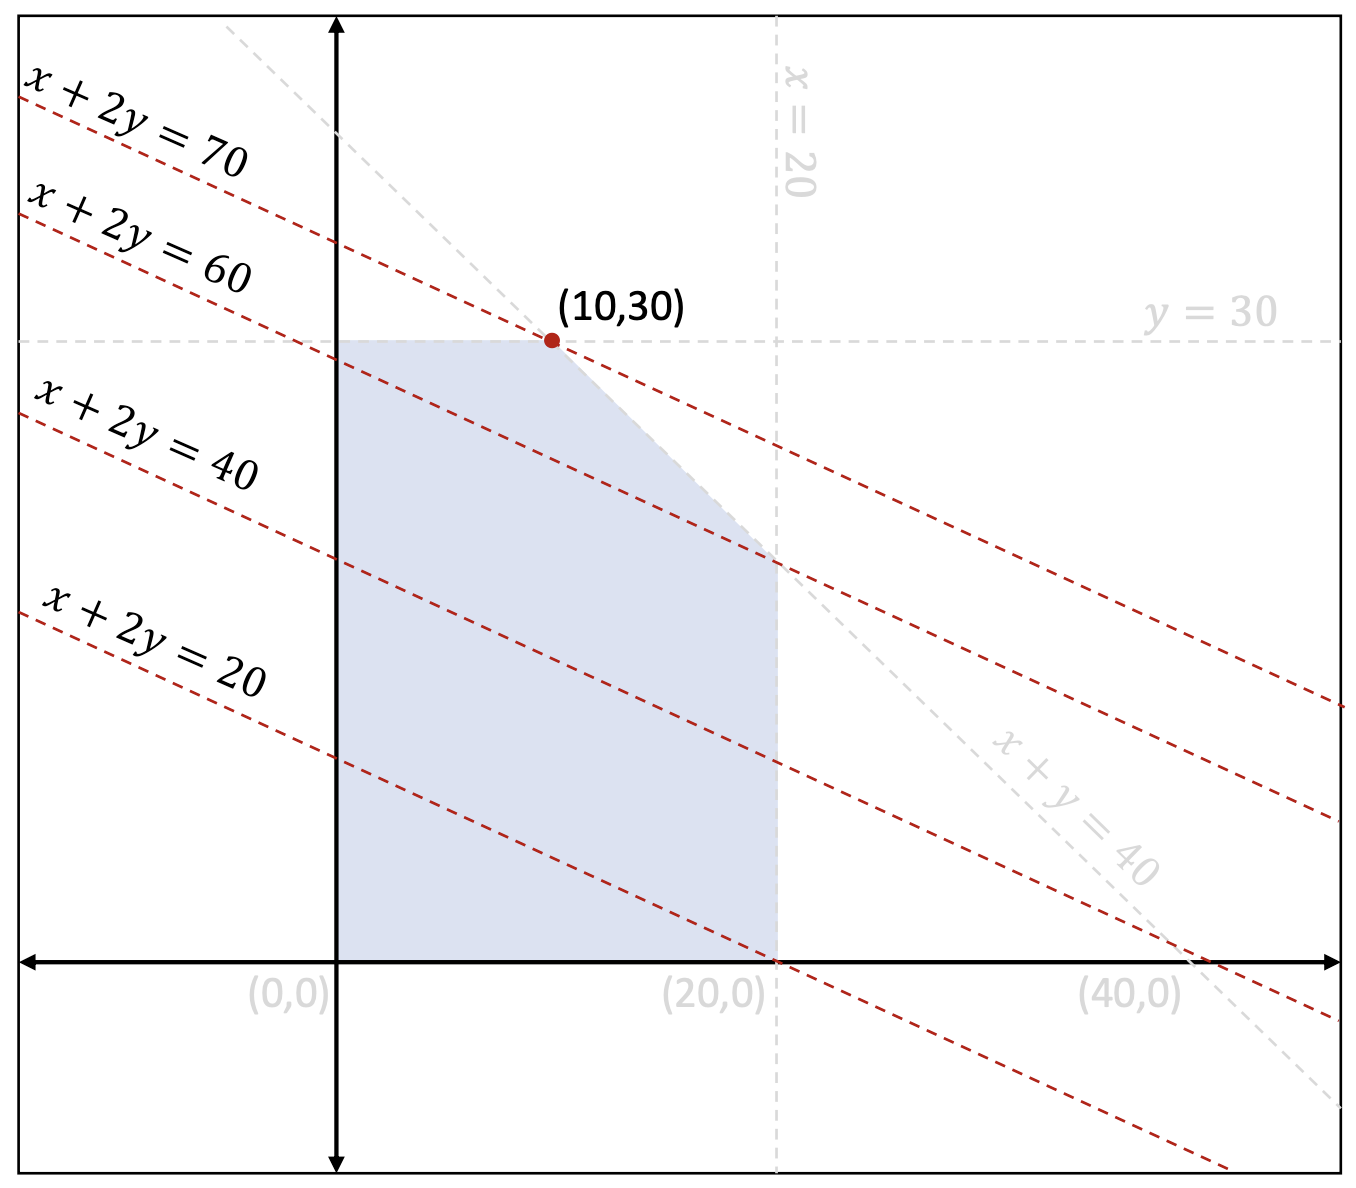
\includegraphics[width=0.7\columnwidth]{L10/find_optimal}
    \end{center}
  \subsection*{Optimal feasible solution DNE}
    \subsubsection*{LP is unbounded}
      \begin{center}
        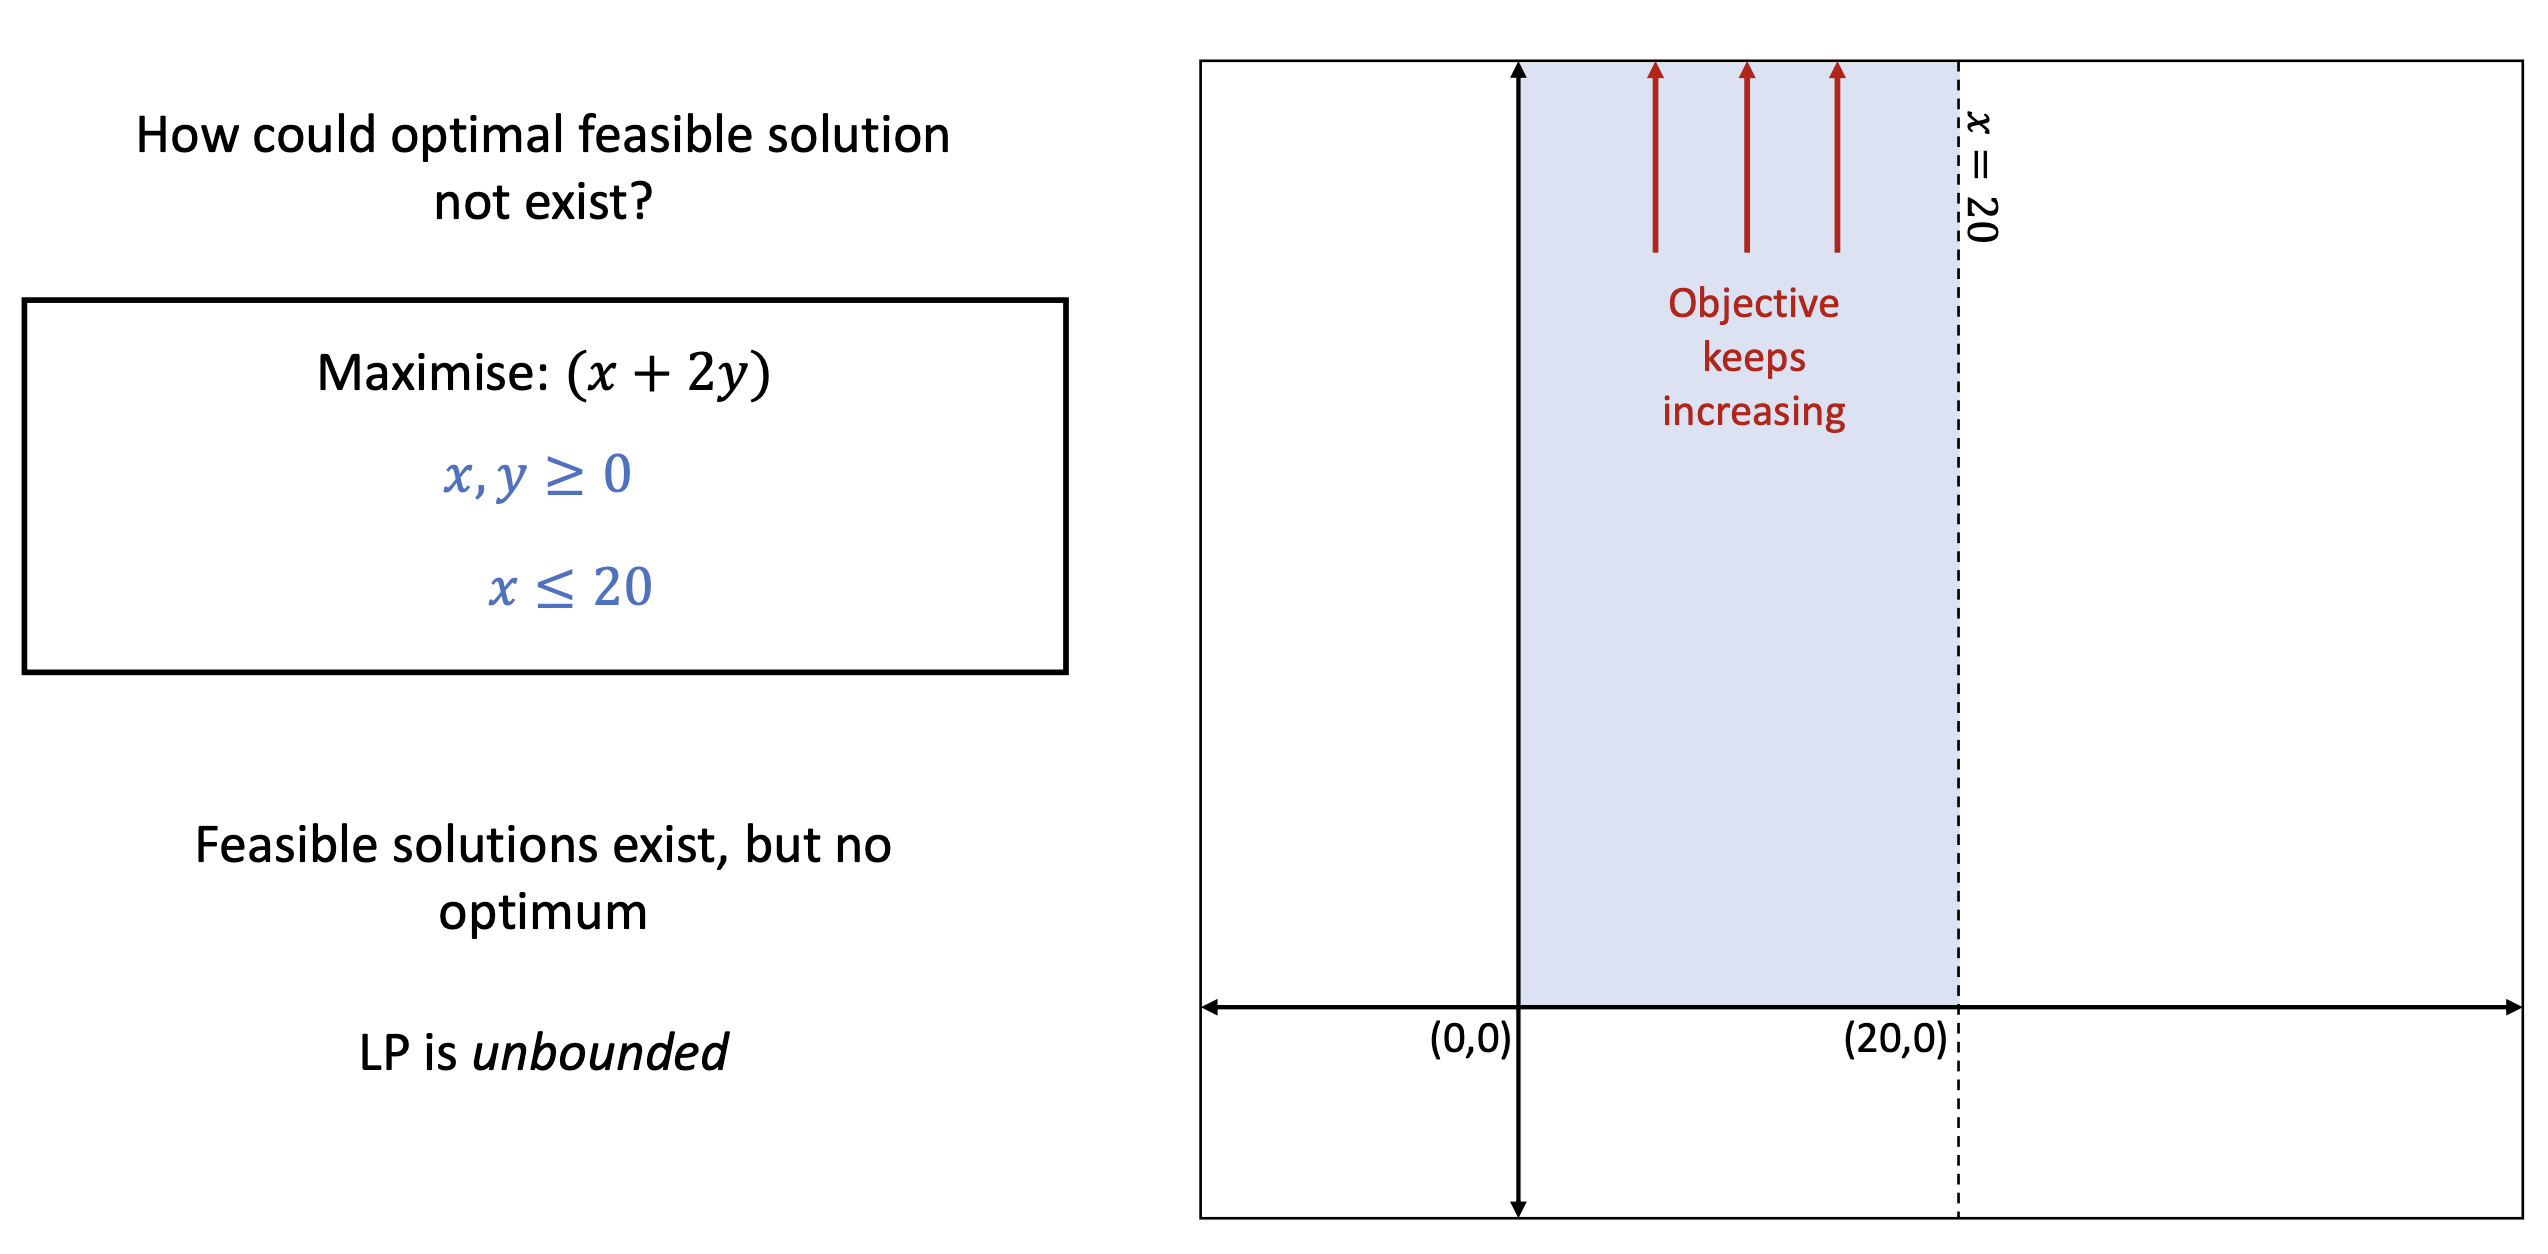
\includegraphics[width=\columnwidth]{L10/unbounded}
      \end{center}
    \subsubsection*{LP is infeasible}
      \begin{center}
        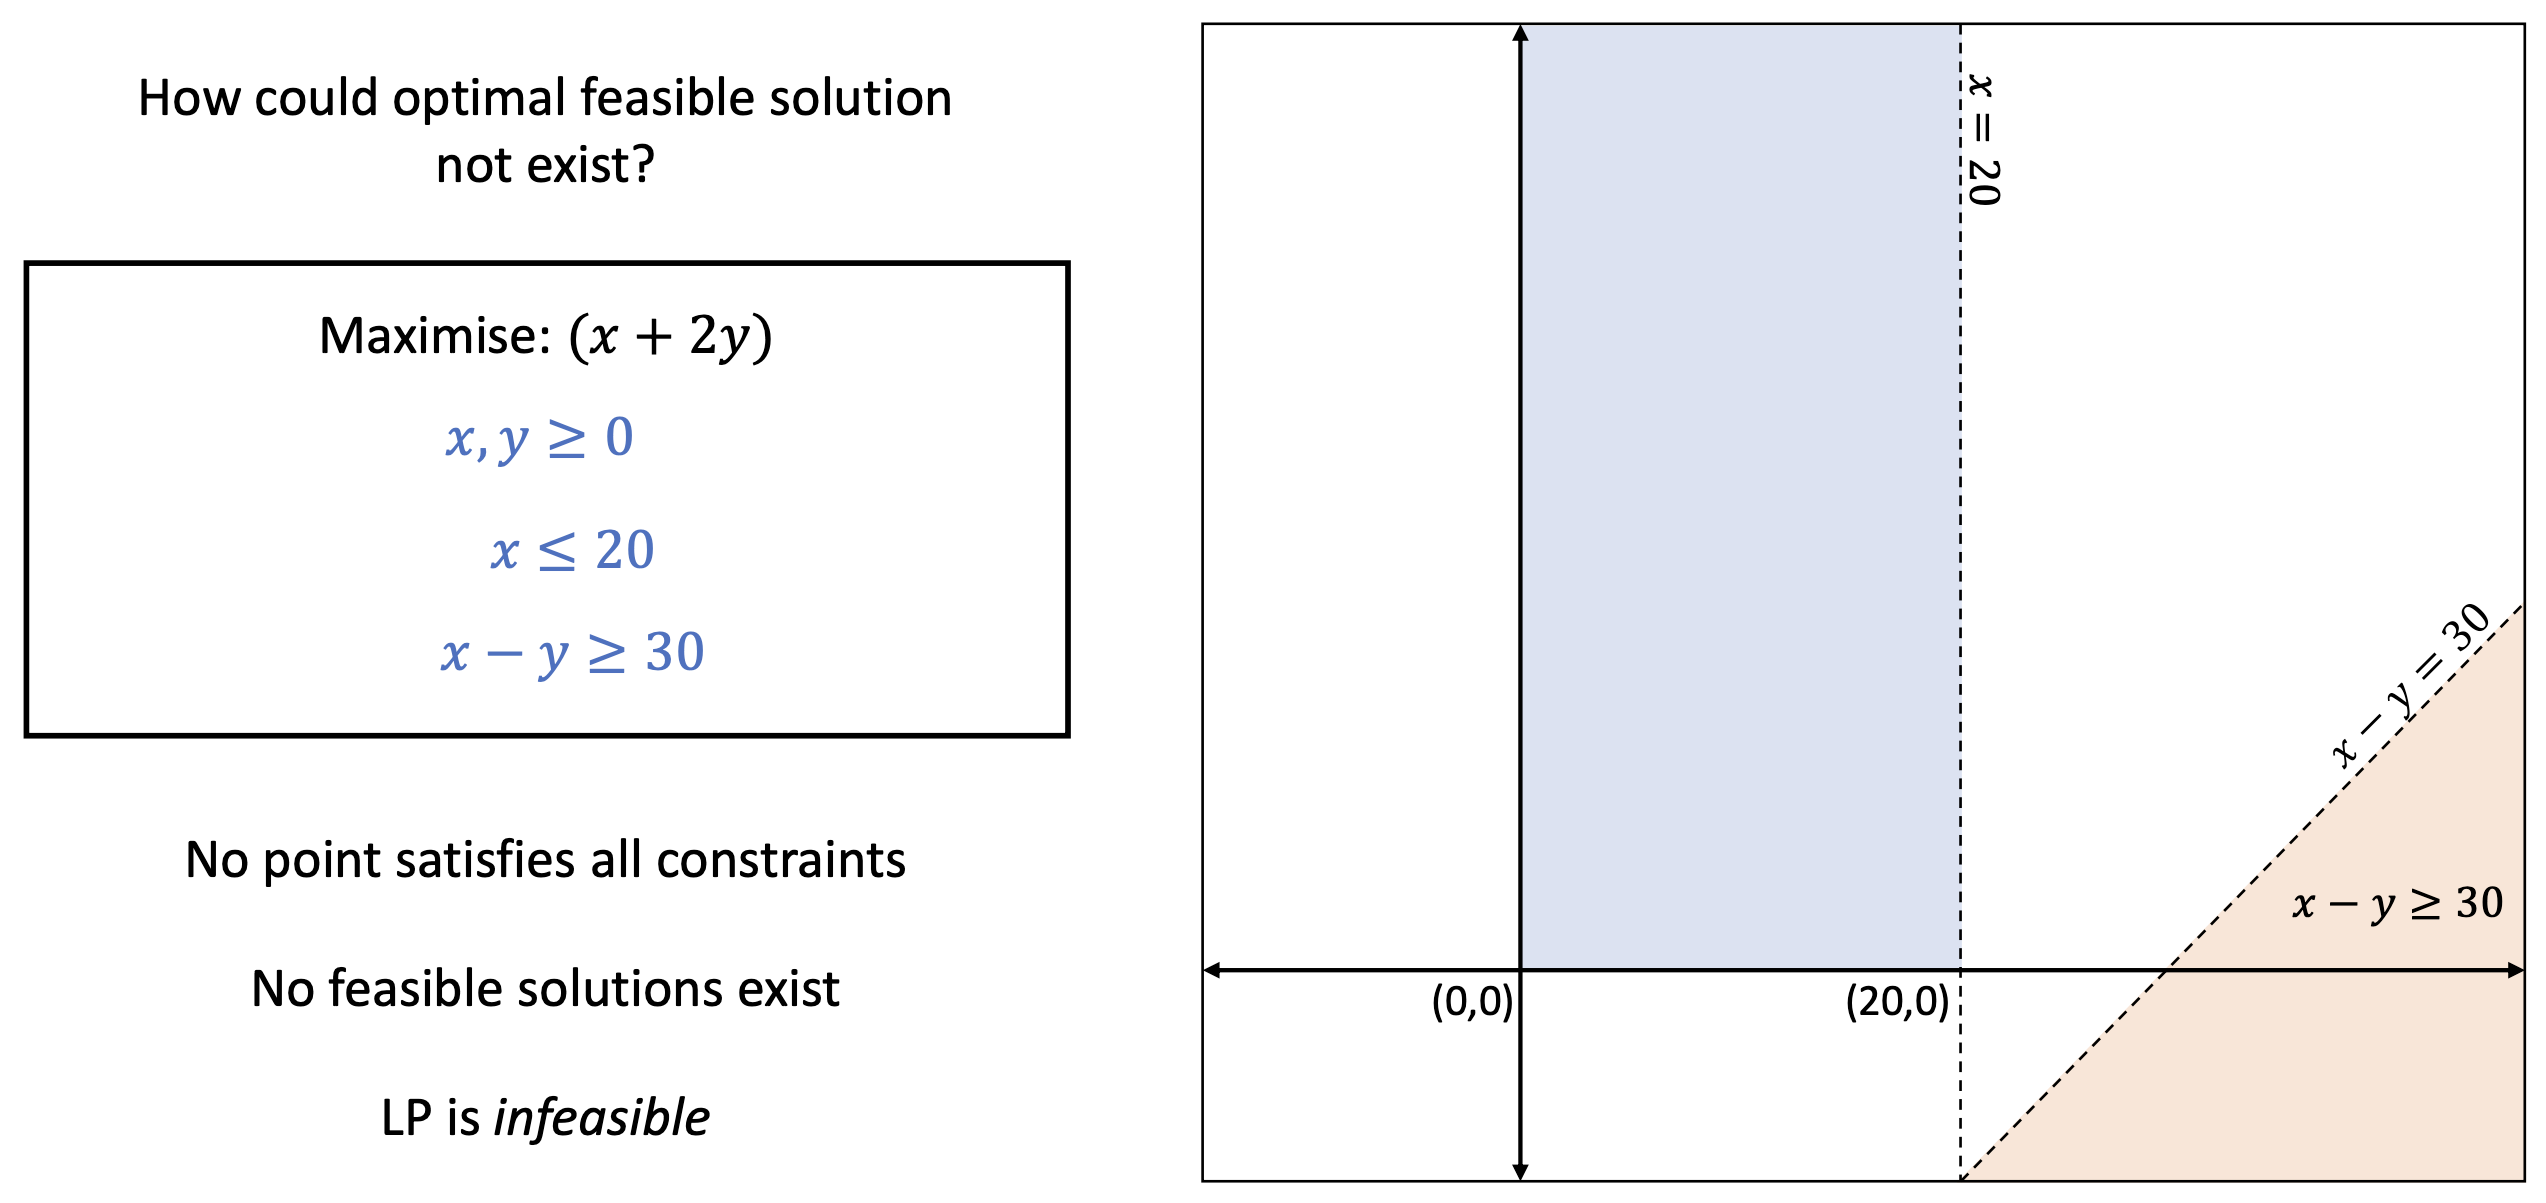
\includegraphics[width=\columnwidth]{L10/infeasible}
      \end{center}
  \subsection*{Simplex algorithm}
    \begin{itemize}[leftmargin=*]
      \item With $n$ variables, the simplex is a $n$-dimensional convex polyhedron
      \item Convex $\implies$ correctness, since any local optimum is a global optimum
      \item Can take exponential time in worst case, but efficient in practice on typical inputs
    \end{itemize}
    \begin{center}
      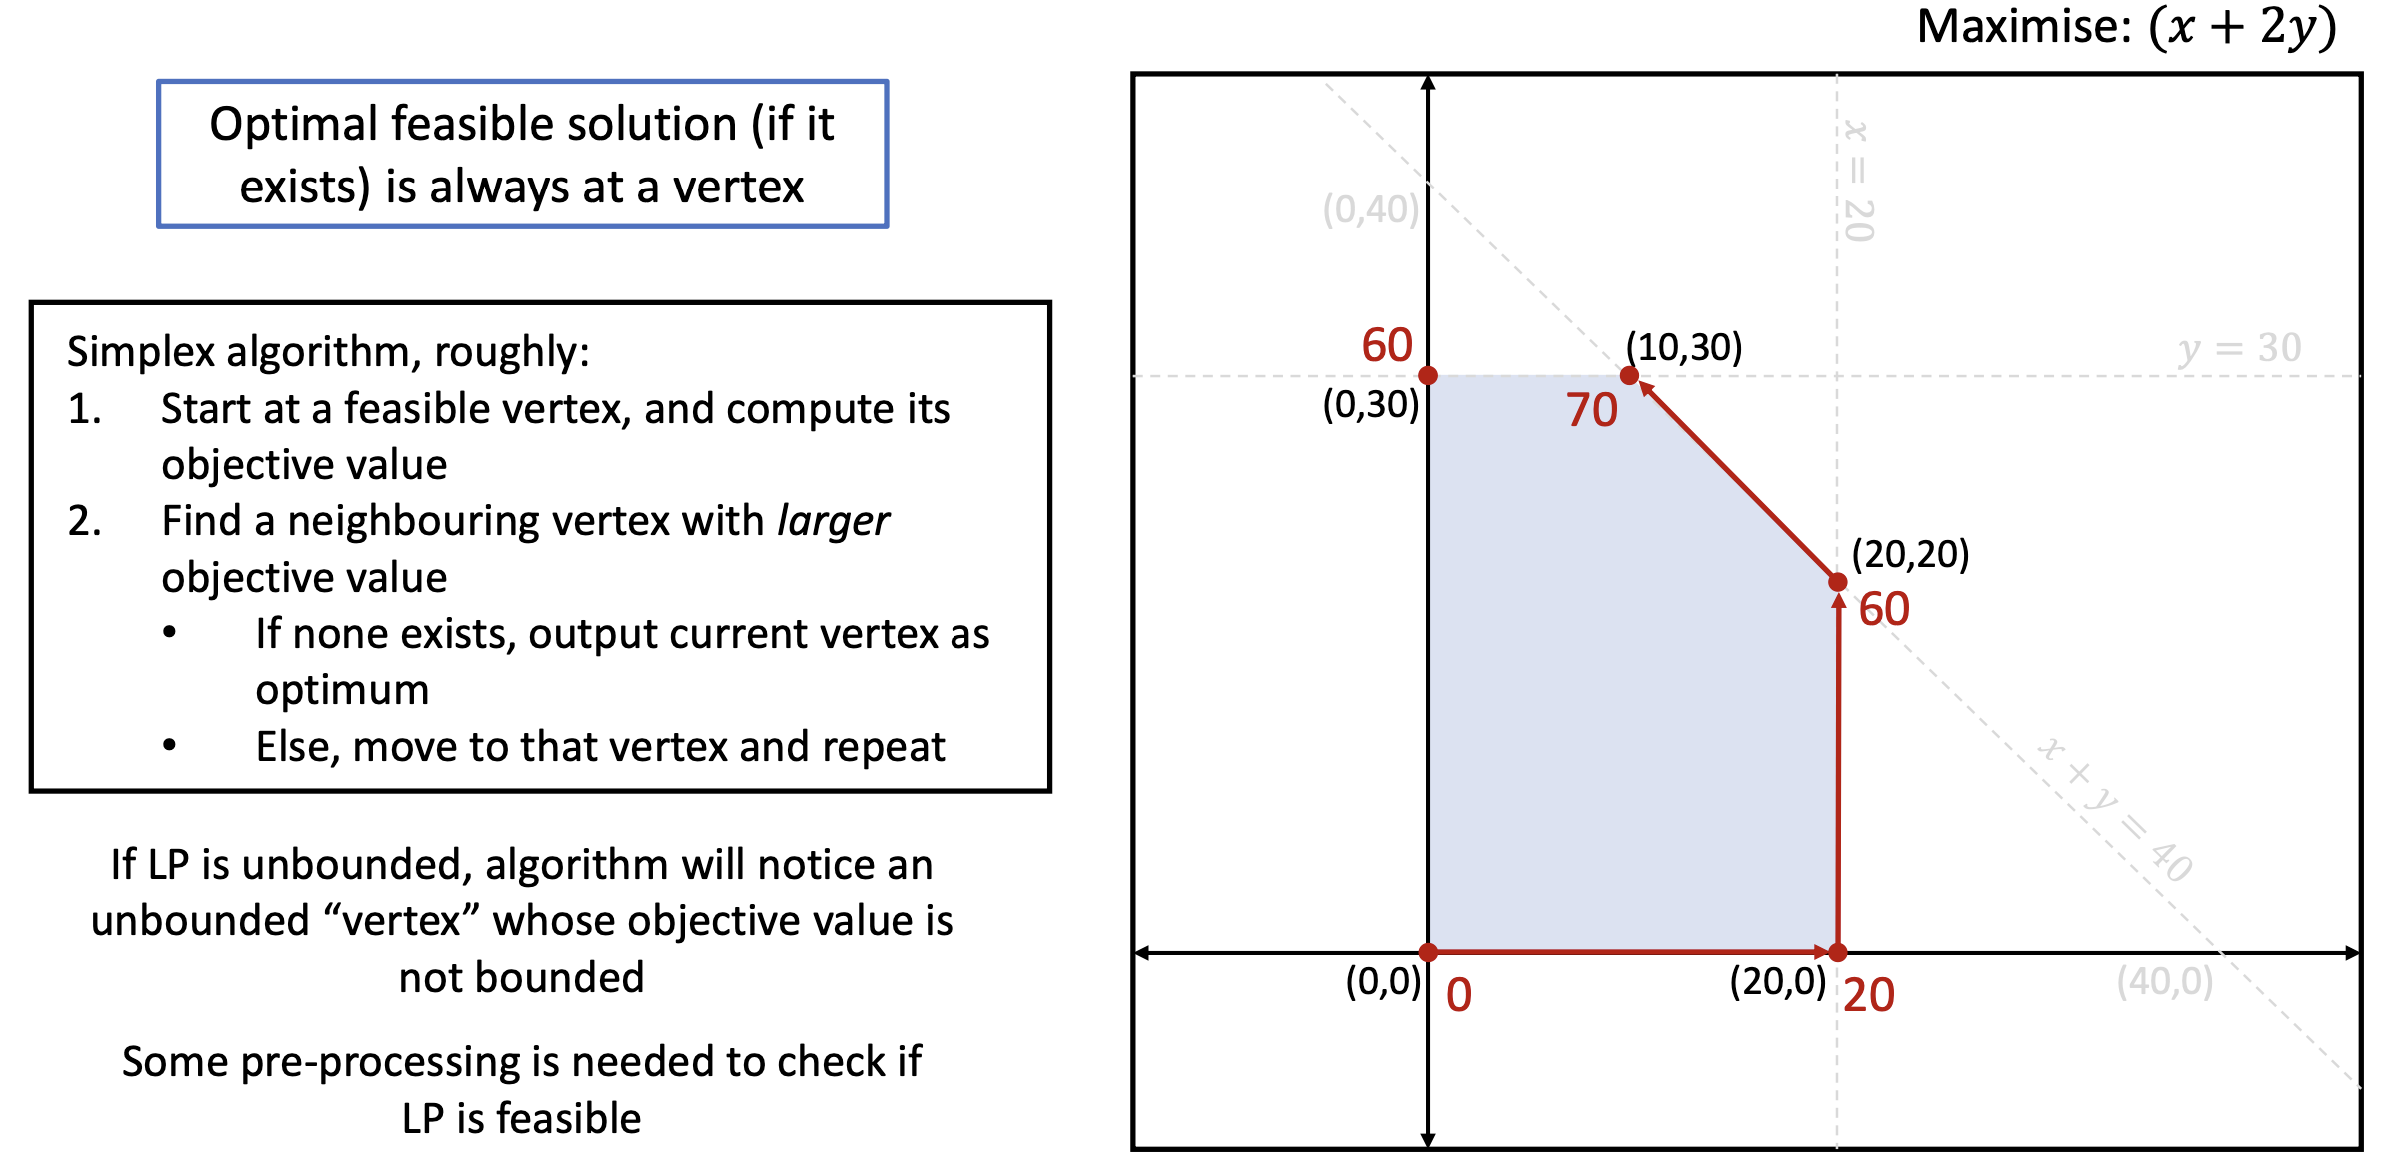
\includegraphics[width=\columnwidth]{L10/simplex_algo}
    \end{center}
\section*{Reductions}
  \subsection*{Reductions} \noindent
    Consider two problems $A$ and $B$. If $A$ can be solved as follows, then we say $A$ reduces to $B$.
    \\\\
    Input: An instance $\alpha$ of $A$
    \begin{enumerate}[leftmargin=*]
      \item Convert $\alpha$ into an instance $\beta$ of $B$
      \item Solve $\beta$ and obtain a solution
      \item Based on the solution of $\beta$, obtain the solution to $\alpha$
    \end{enumerate}
    \begin{center}
      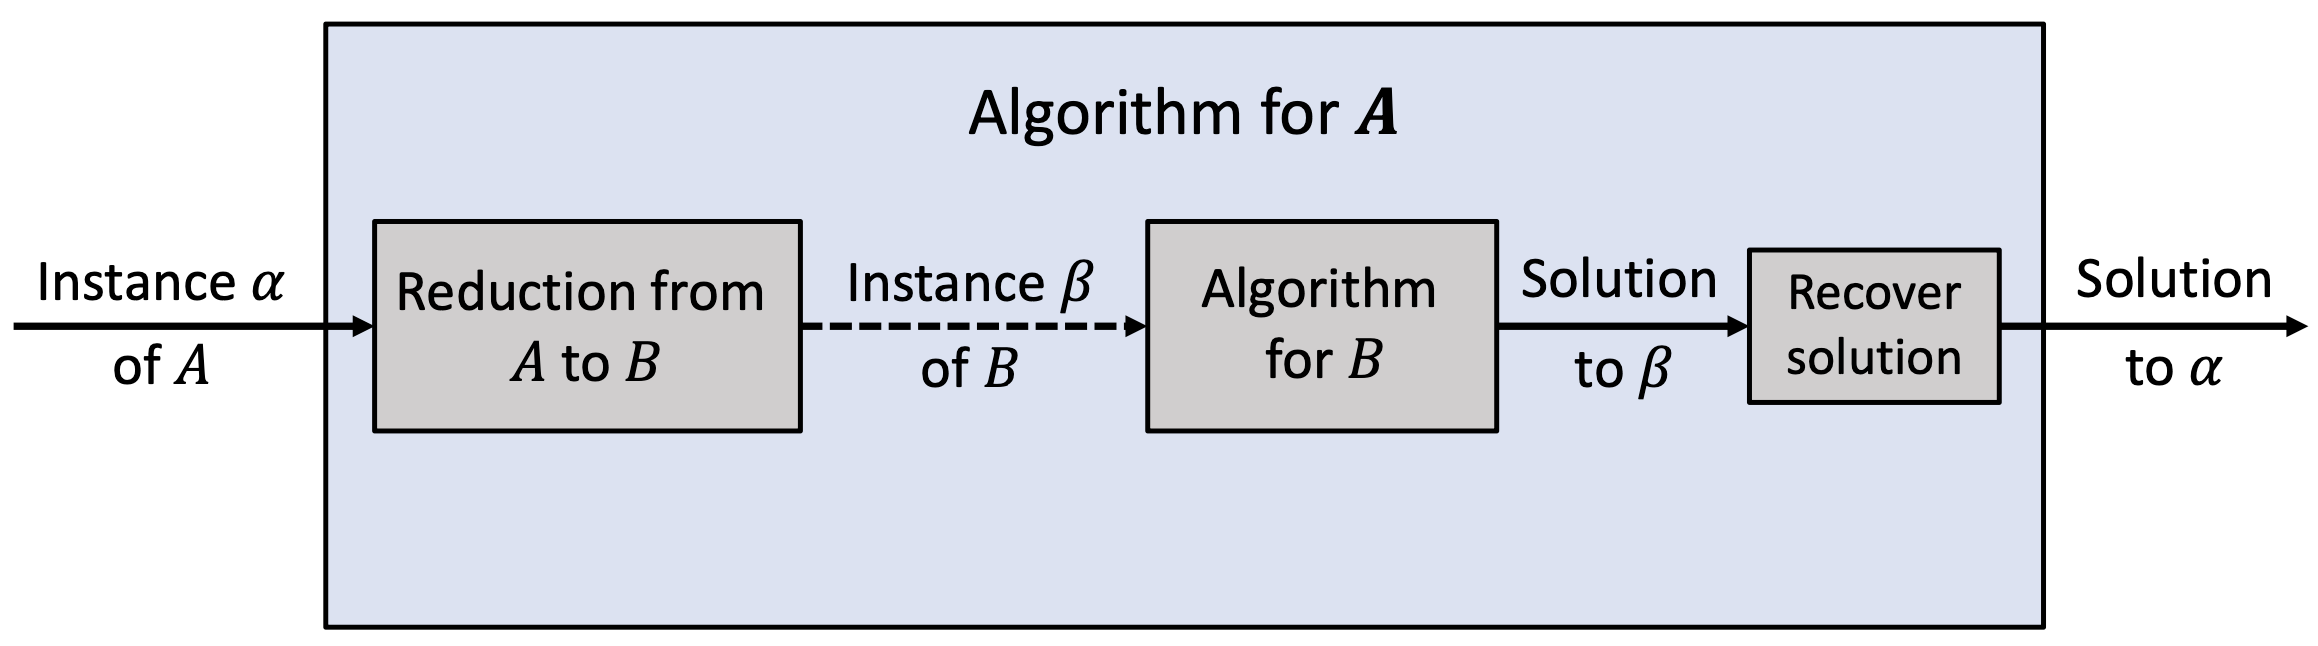
\includegraphics[width=\columnwidth]{L11/reduction}
    \end{center}
    \subsubsection*{Bounded-time reduction} \noindent
      Consider two problems $A$ and $B$, and a function $p$. If $A$ can be solved as follows, then we say $A$ has a $p(n)$-time reduction to $B$.
      \\\\
      Input: An instance $\alpha$ of $A$ of size $n$
      \begin{enumerate}[leftmargin=*]
        \item Convert $\alpha$ into an instance $\beta$ of $B$ in $p(n)$ time
        \item Solve $\beta$ and obtain a solution
        \item Based on the solution of $\beta$, obtain the solution to $\alpha$ in $p(n)$ time
      \end{enumerate}
      \begin{center}
        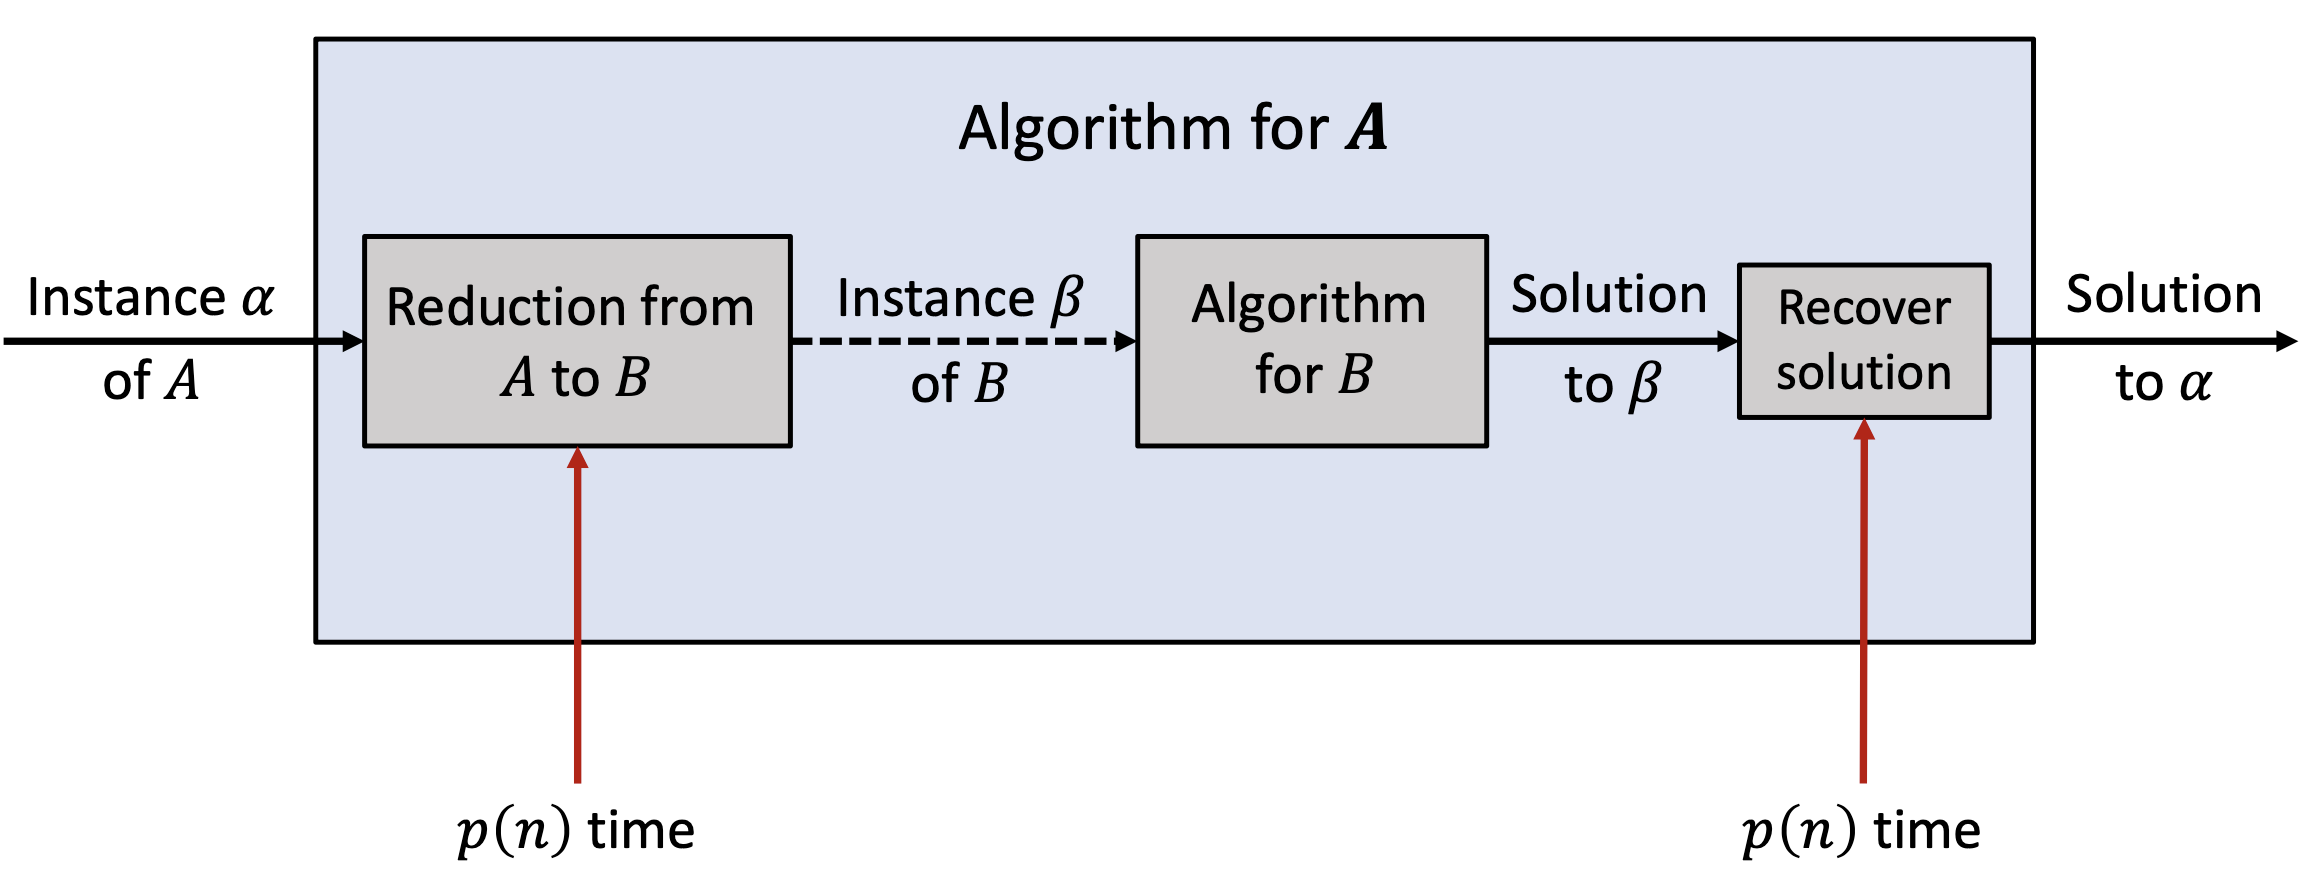
\includegraphics[width=\columnwidth]{L11/bounded_time_reduction}
      \end{center}
    \subsubsection*{Problem instance size}
      \begin{itemize}[leftmargin=*]
        \item $n$ is the length of the encoding of the problem instance. It is roughly the number of bits used to write down that instance
        \item Can use standard encoding for many problems
          \begin{itemize}[leftmargin=*]
            \item Integers: Binary encoding
            \item Graphs, matrices: List of parameters enclosed by braces, separated by commas
          \end{itemize}
      \end{itemize}
  \subsection*{Running time}
    \subsubsection*{Running time composition} \noindent
      If there is
      \begin{itemize}[leftmargin=*]
        \item a $p(n)$-time reduction from problem $A$ to problem $B$, and
        \item a $T(n)$-time algorithm to solve problem $B$ on instances of size $n$
      \end{itemize}
      then there is a
      \[ T(p(n)) + O(p(n)) \]
      time algorithm to solve problem $A$ on instances of size $n$
      \begin{center}
        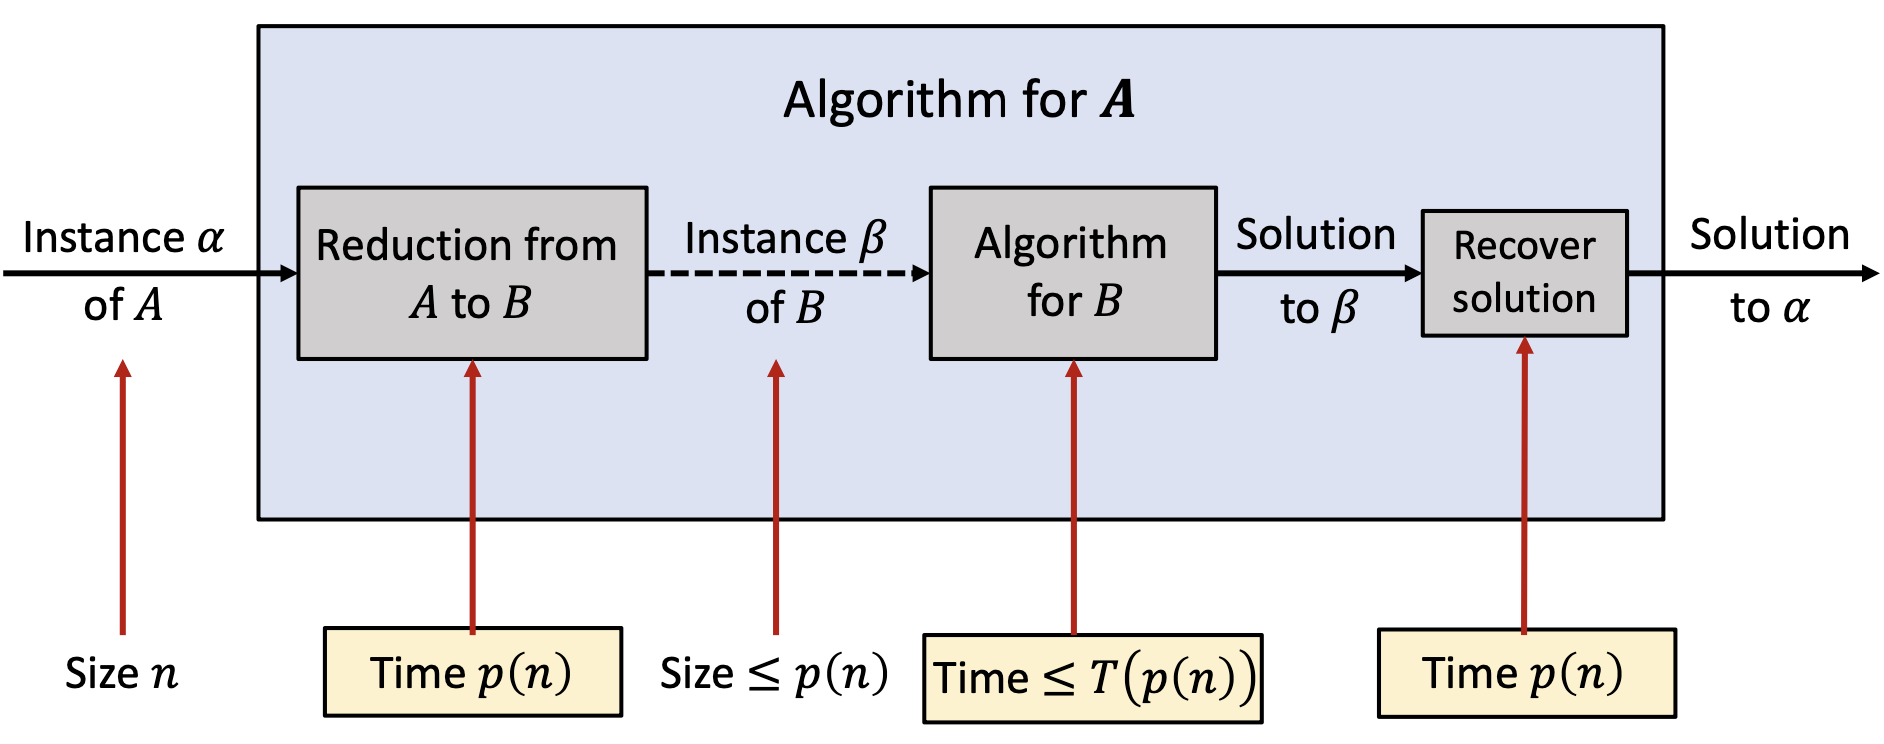
\includegraphics[width=\columnwidth]{L11/running_time_composition}
      \end{center}
    \subsubsection*{Polynomial-time reduction} \noindent
      $A \leq_P B$ if there is a $p(n)$-time reduction from $A$ to $B$ for some polynomial function $p(n)$
      \begin{itemize}[leftmargin=*]
        \item If $B$ has a polynomial time algorithm, then so does $A$
        \item If $A$ cannot be solved in polynomial time, then neither can $B$
      \end{itemize}
    \subsubsection*{Pseudo-polynomial algorithms} \noindent
      An algorithm that runs in time
      \begin{itemize}[leftmargin=*]
        \item polynomial in the numeric value of the input, but
        \item exponential in the length of the representation of the input
      \end{itemize}
  \subsection*{Intractability}
    \subsubsection*{Decision vs Optimization}
      \begin{itemize}[leftmargin=*]
        \item A \uline{decision problem} is a function that maps each instance to either YES or NO
        \item \uline{Decision reduces to optimization.} Given an instance of the optimization problem and a number $k$, ask whether there is a solution with value $\leq k$
      \end{itemize}
    \subsubsection*{\yellow{Reductions between decision problems}}
      \begin{center}
        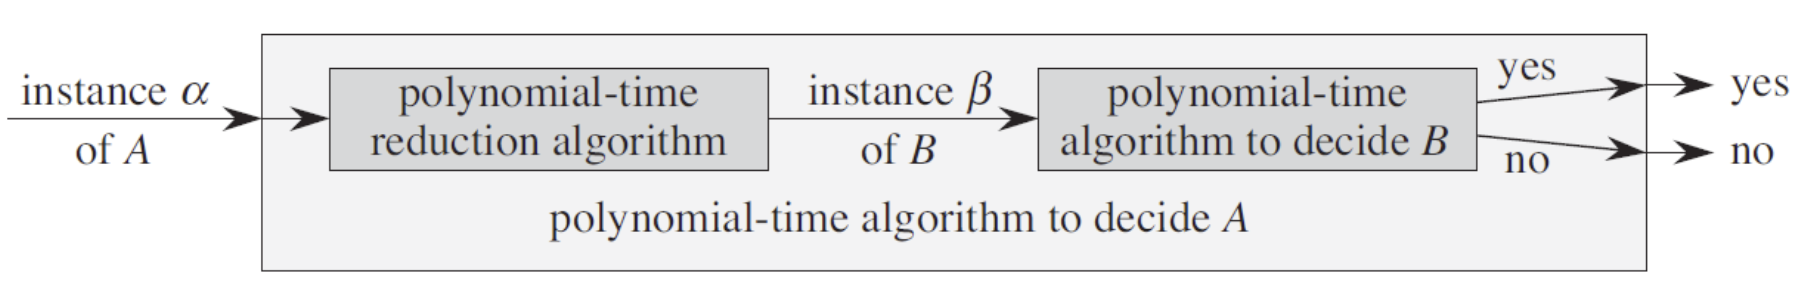
\includegraphics[width=\columnwidth]{L11/decision_problems}
      \end{center}
      Suffices to show:
      \begin{itemize}[leftmargin=*]
        \item Reduction runs in polynomial time
        \item If $\alpha$ is a YES-instance of $A$, $\beta$ is a YES-instance of $B$
        \item If $\beta$ is a YES-instance of $B$, $\alpha$ is a YES-instance of $A$
      \end{itemize}
\section*{NP-Completeness}
  \subsection*{Reduction chart} \noindent
    Note the the arrow points in the direction of the reduction
    \begin{center}
      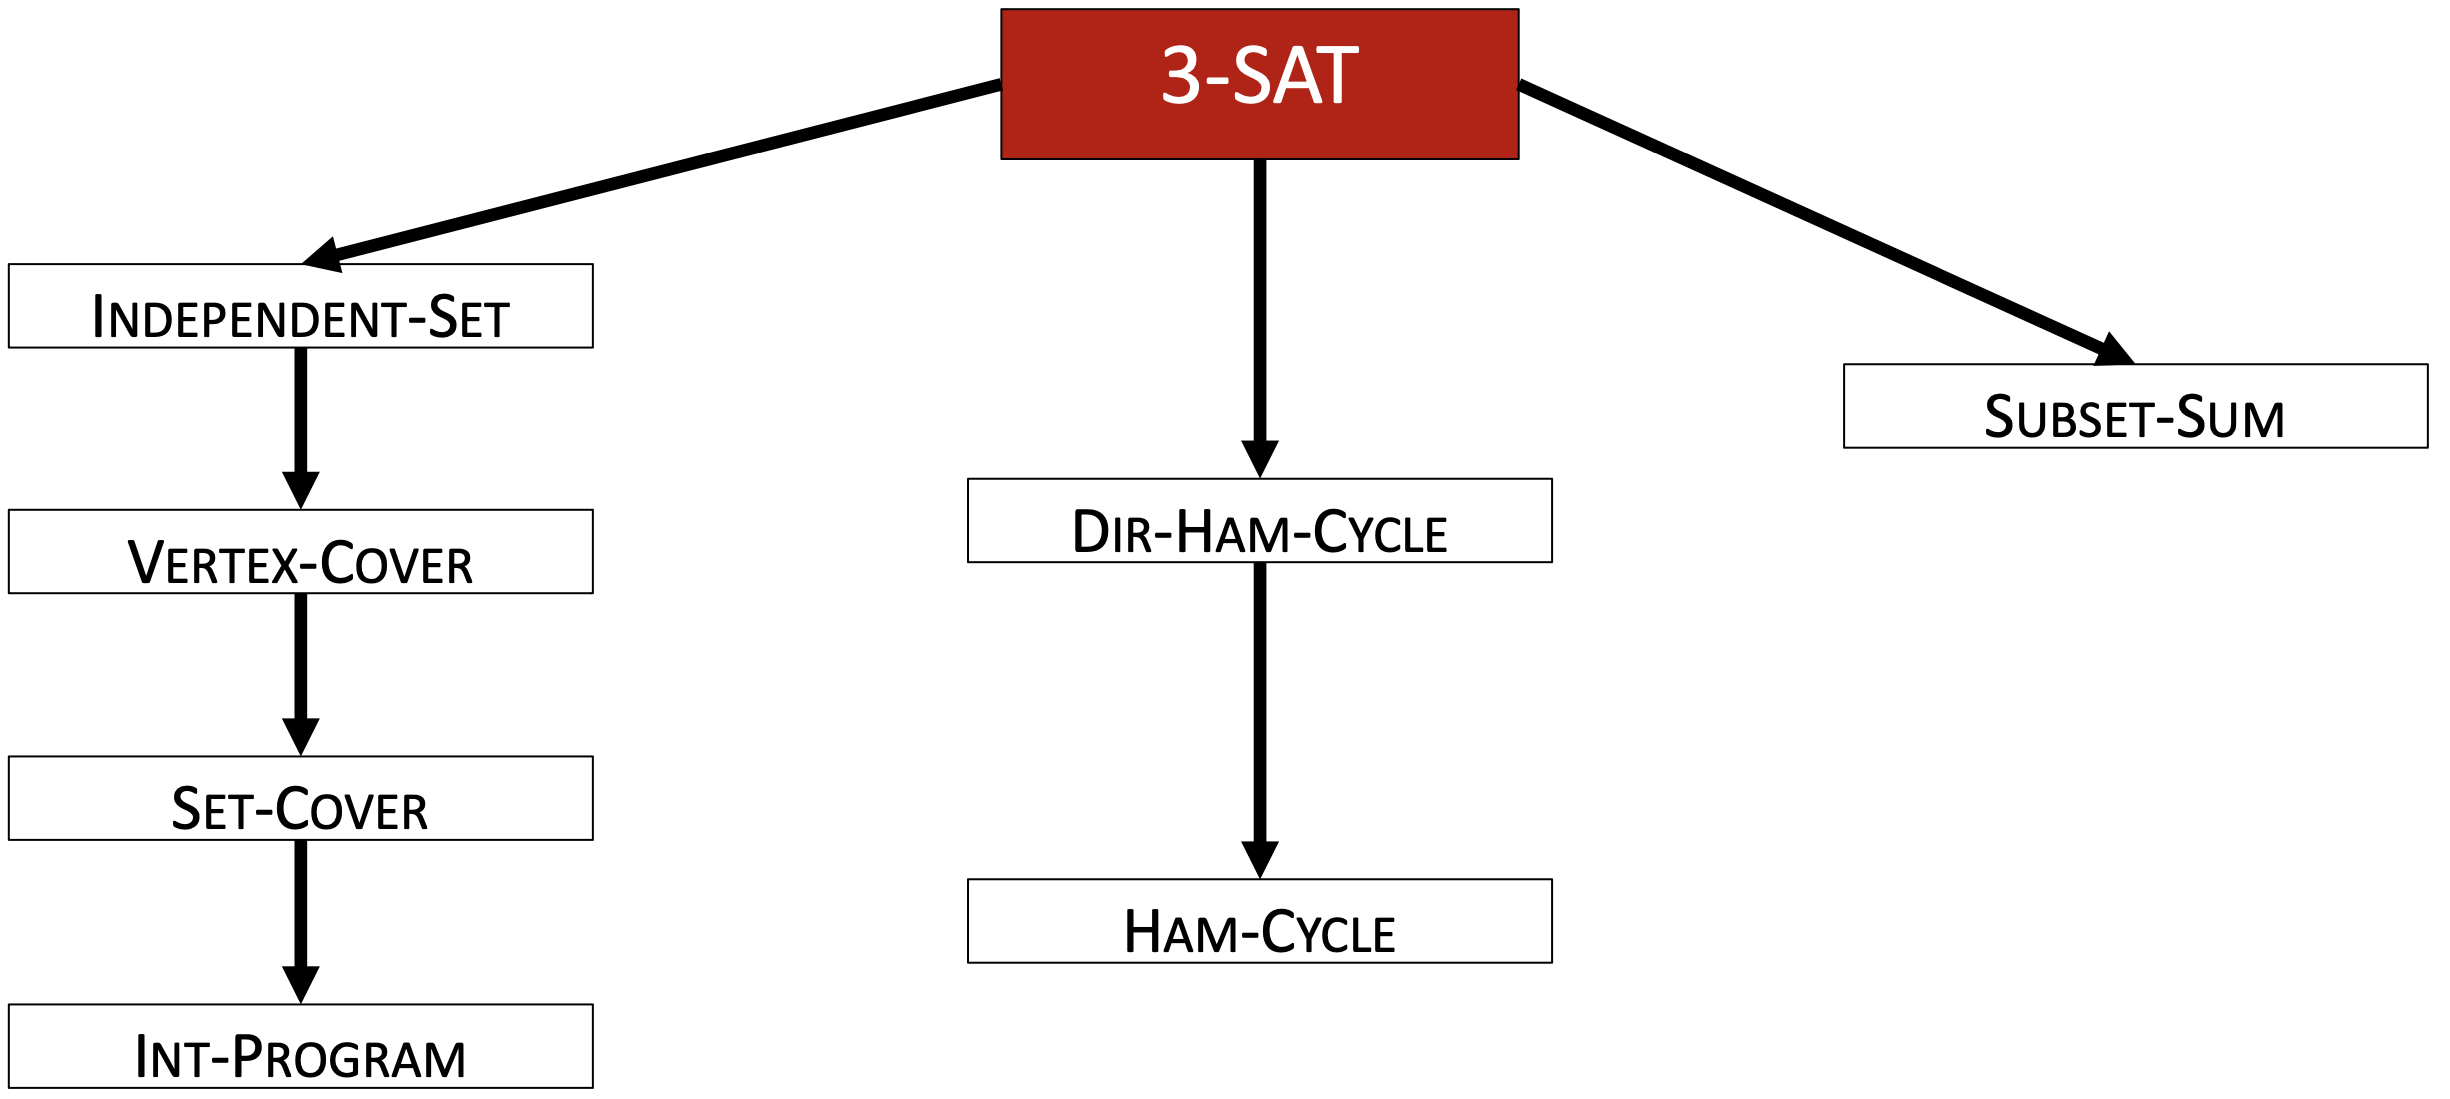
\includegraphics[width=\columnwidth]{L12/reduction_chart}
    \end{center}
    3-SAT is NP-hard and NP-complete, and so are the other problems in this chart.
  \subsection*{Problem definitions}
    \subsubsection*{Independent-Set} \noindent
      Given a graph $G=(V,E)$ and an integer $k$, is there a subset of $\geq k$ vertices such that no two are adjacent?
    \subsubsection*{Vertex-Cover} \noindent
      Given a graph $G=(V,E)$ and an integer $k$, is there a subset of $\leq k$ vertices such that each edge is incident to at least one vertex in the subset?
      \begin{center}
        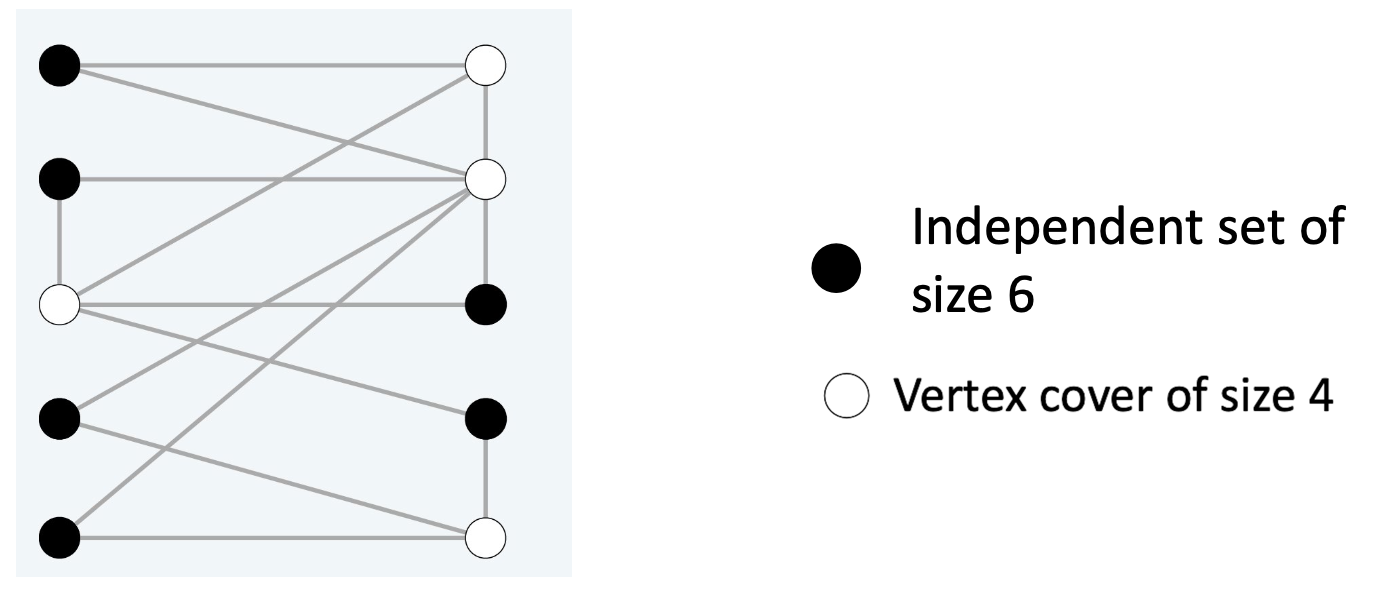
\includegraphics[width=\columnwidth]{L12/independent_set}
      \end{center}
    \subsubsection*{Set-Cover} \noindent
      Given integers $k$ and $n$, and a collection $\mathcal{S}$ of subsets of $\{1, \cdots, n\}$, are there $\leq k$ of these subsets whose union equal $\{1, \cdots, n\}$?
      \begin{center}
        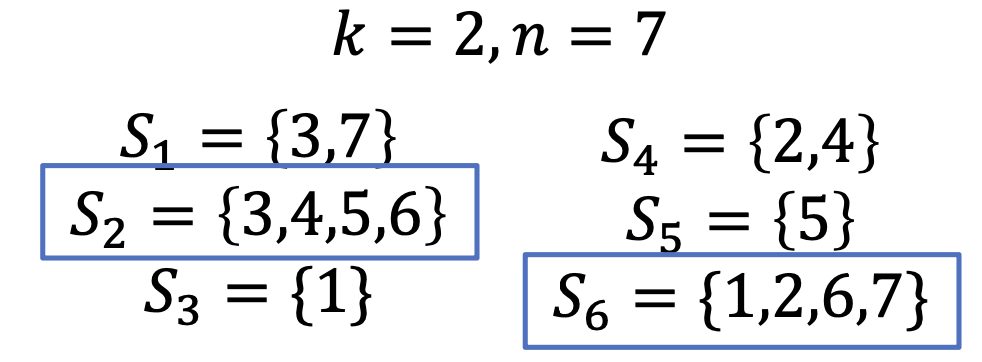
\includegraphics[width=0.8\columnwidth]{L12/set_cover}
      \end{center}
    \subsubsection*{3-SAT} \noindent
      \begin{itemize}[leftmargin=*]
        \item Boolean variable: a variable that takes values True or False
        \item Literal: a Boolean variable or its negation
        \item Clause: a disjunction (OR) of literals, e.g. $C_j = x_1 \lor \bar{x}_2 \lor x_3$
        \item Conjunctive Normal Form (CNF) formula: a formula that is a conjunction (AND) of clauses
        \item Satifsying assignment: an assignment of $x_i$ that makes the formula evaluate to True
      \end{itemize}
      Given a CNF formula $\phi$ over $n$ variables, does it have a satisfying assignment?
    \subsubsection*{Integer-Program} \noindent
      Given a set of $m$ linear constraints in $n$ variables
      \begin{gather*}
        a_{11} x_1 + \cdots + a_{1n} x_n \leq b_1 \\
        \cdots \\
        a_{m1} x_1 + \cdots + a_{mn} x_n \leq b_m
      \end{gather*}
      is there an assignment of values $\{0, 1\}$ to the $x_i$ such that all the constraints are satisified
      \begin{itemize}[leftmargin=*]
        \item Essentially a LP with additional constraint that each $x_i \in \{0, 1\}$
      \end{itemize}
    \subsubsection*{Subset-Sum} \noindent
      Given a list of integers $S$ and a target $t$, decide if there is $S' \subseteq S$ that sums up to $t$.
    \subsubsection*{Dir-Ham-Cycle} \noindent
      Given a directed graph $G=(V,E)$, is there a simple directed cycle $\Gamma$ that contains every node in $V$ exactly once?
      \begin{center}
        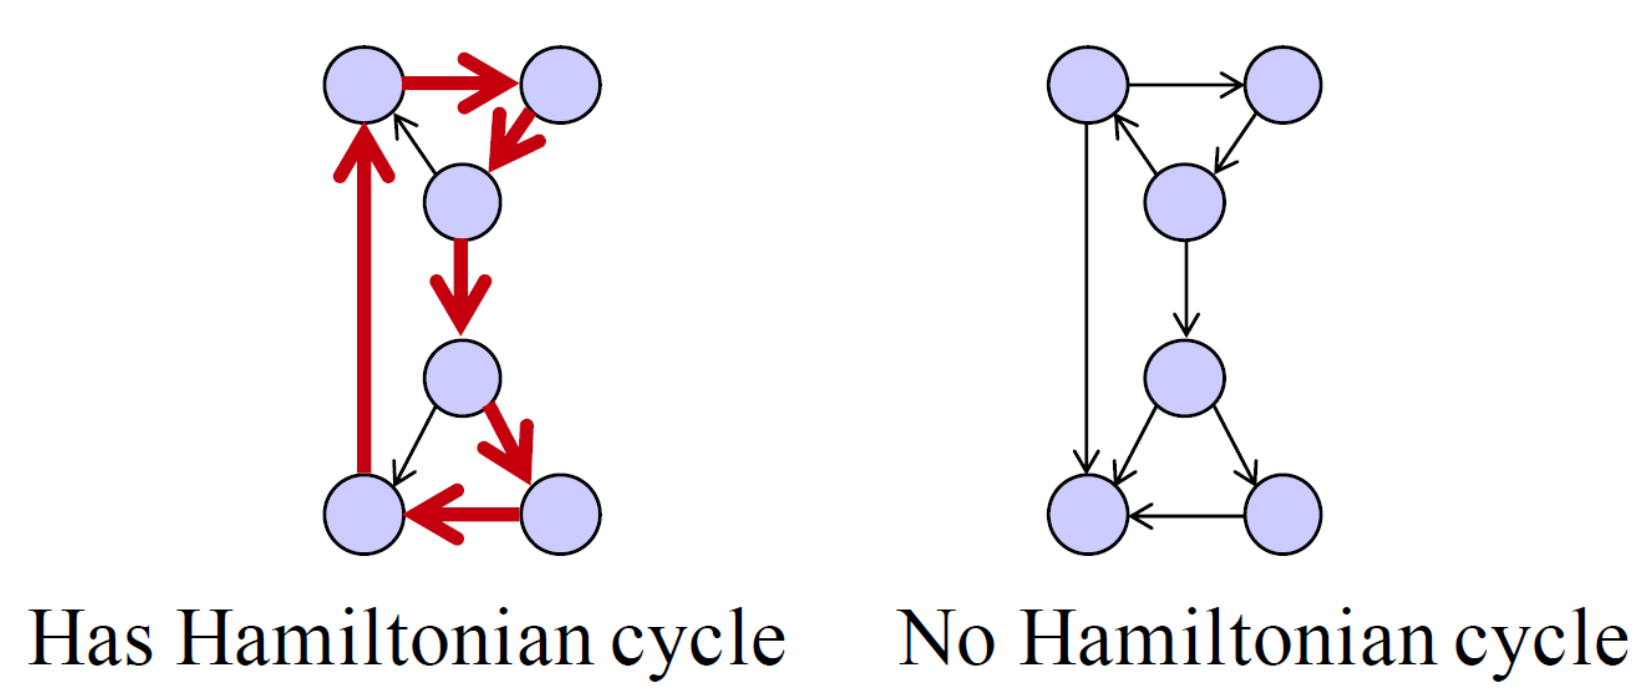
\includegraphics[width=0.8\columnwidth]{L12/dir_ham_cycle}
      \end{center}
    \subsubsection*{Ham-Cycle} \noindent
      Given an undirected graph $G=(V,E)$, is there a simple cycle that contains every node in $V$ exactly once?
\section*{Complexity classes}
  \begin{center}
    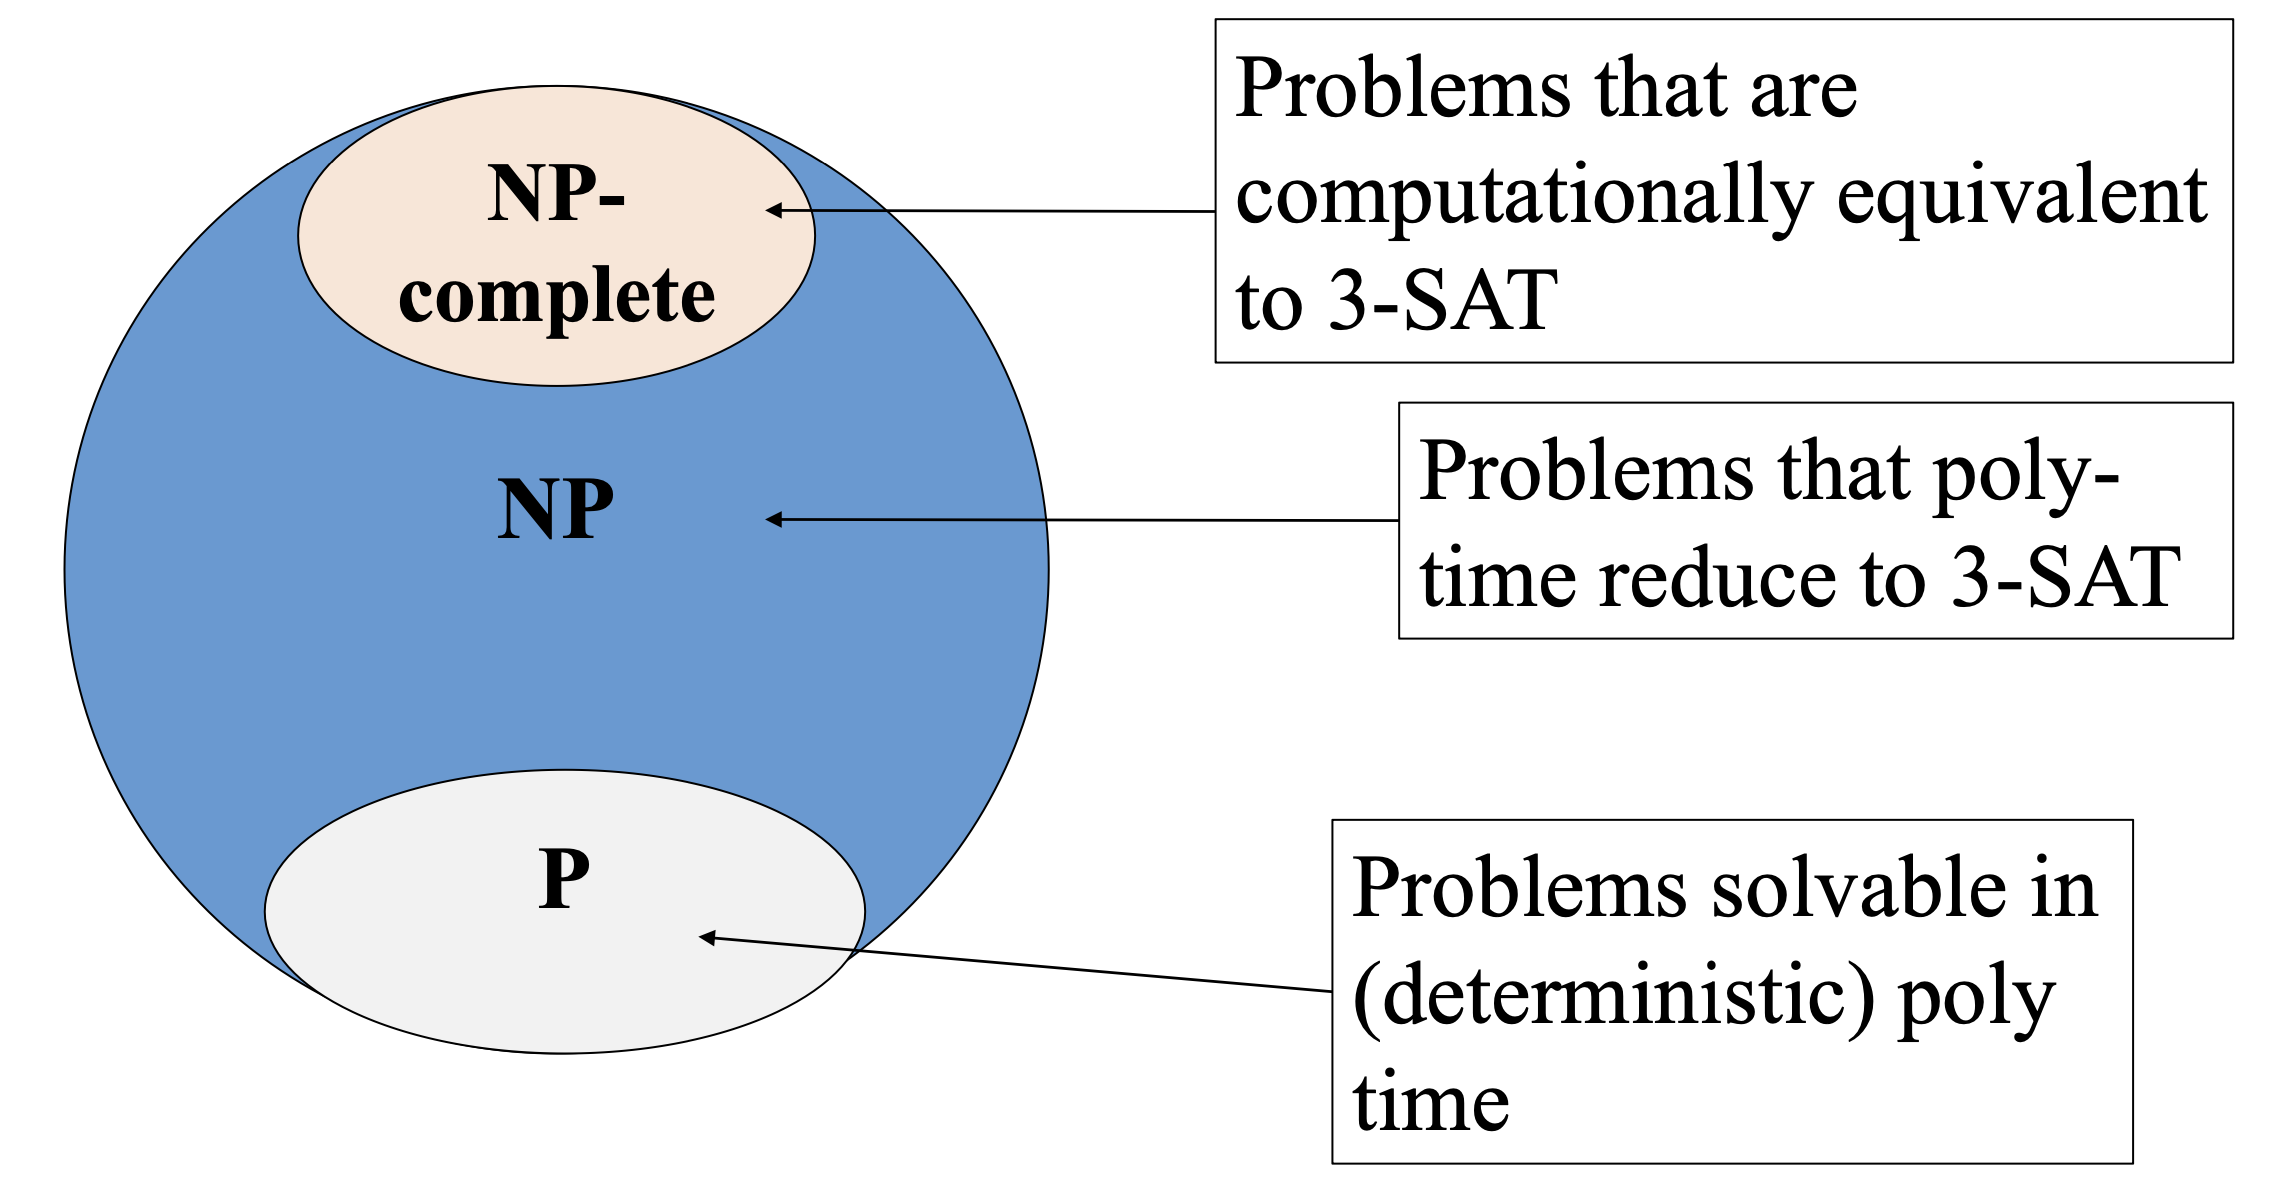
\includegraphics[width=\columnwidth]{L12/complexity_classes}
  \end{center}
  \subsection*{Some problems in P}
    \begin{center}
      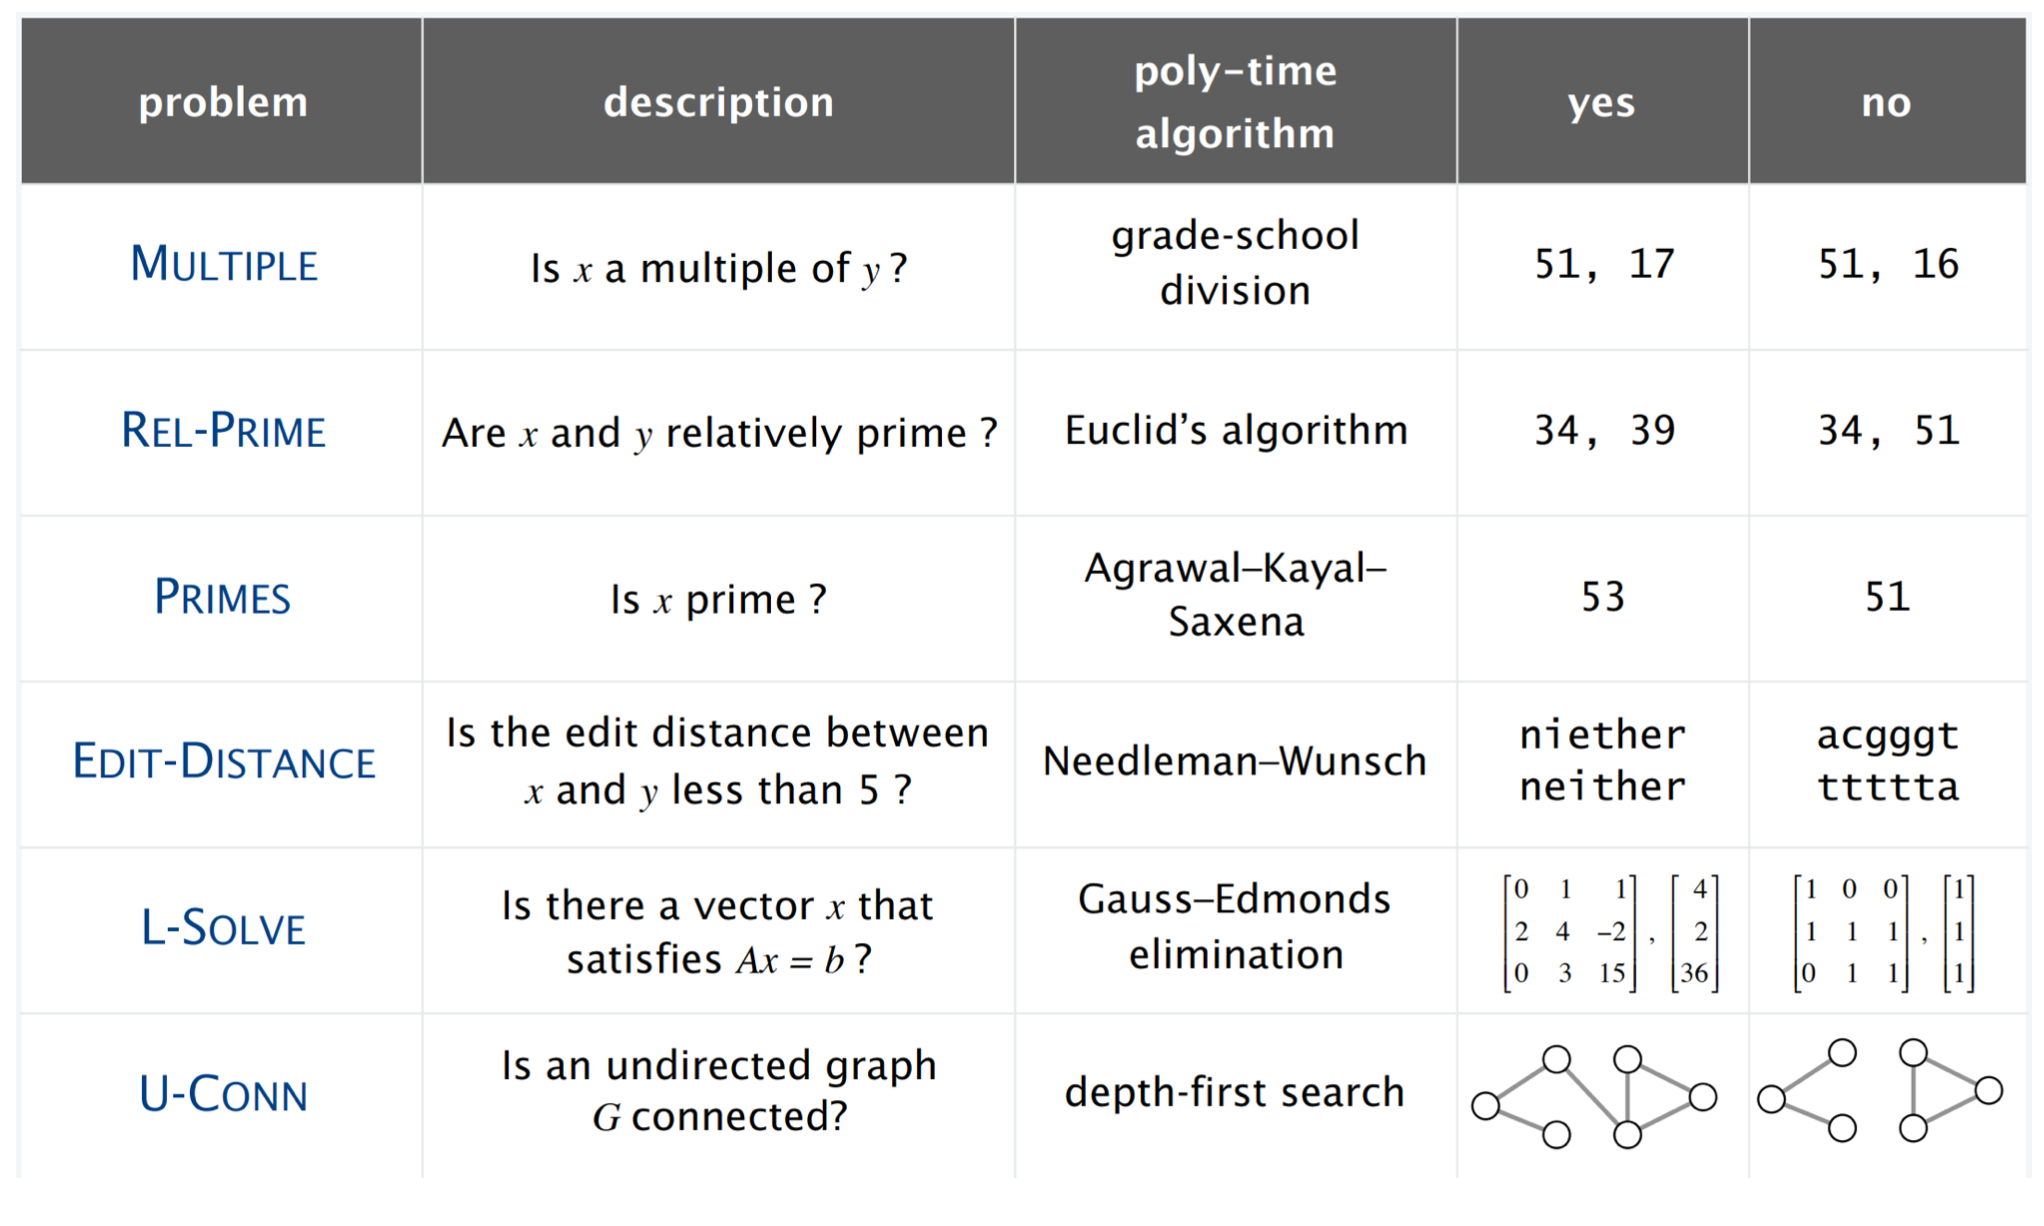
\includegraphics[width=\columnwidth]{L12/problems_in_p}
    \end{center}
    \vspace{-0.5cm}
  \subsection*{NP}
    \begin{itemize}[leftmargin=*]
      \item Short for non-deterministic polynomial
      \item Defined as the class of problems for which polynomial time verifiable certs of YES-instances exist
      \item There is a verification algo $V(x,y)$ that takes in an instance $x$ and certificate $y$ with $\lvert y \rvert = poly(\lvert x \rvert)$ such that
        \[ \exists y \text{ s.t. } V(x,y) = 1 \iff x \text{ is a YES-instance} \]
      \item P $\subseteq$ NP because certificate can be anything, while verifier $V(x, \cdot)$ can solve for the instance $x$ by itself and check if it is a YES-instance
    \end{itemize}
    \paragraph{Subset-Sum} Certificate is the subset $S' \subseteq S$ that sums up to $T$. Verifier checks whether the sum of elements of $S'$ is $t$, in polynomial time. Hence Subset-Sum is in NP.
  \subsection*{co-NP}
    \begin{itemize}[leftmargin=*]
      \item A problem is in co-NP if polynomial time verifiable certificates of NO-instances exist
      \item The complement of any NP problem is in co-NP
    \end{itemize}
  \subsection*{NP-Hard} \noindent
    A problem $A$ is said to be NP-Hard if for any problem $B$ in NP,
    \[ B \leq_P A \]
  \subsection*{\yellow{Show NP-Complete}} \noindent
    \begin{itemize}[leftmargin=*]
      \item Show that the problem is in NP, i.e. has a polynomial time verifiable certificate of YES-instance
      \item Show that the problem is in NP-hard, i.e. reduce FROM some known NP-hard problem TO this problem
    \end{itemize}
  \subsection*{Relationships}
    \subsubsection*{Cook-Levin Theorem} \noindent
      Any problem in NP poly-time reduces to 3-SAT. Hence, 3-SAT is NP-hard and NP-complete.
    \subsubsection*{Likely relationships}
      \begin{center}
        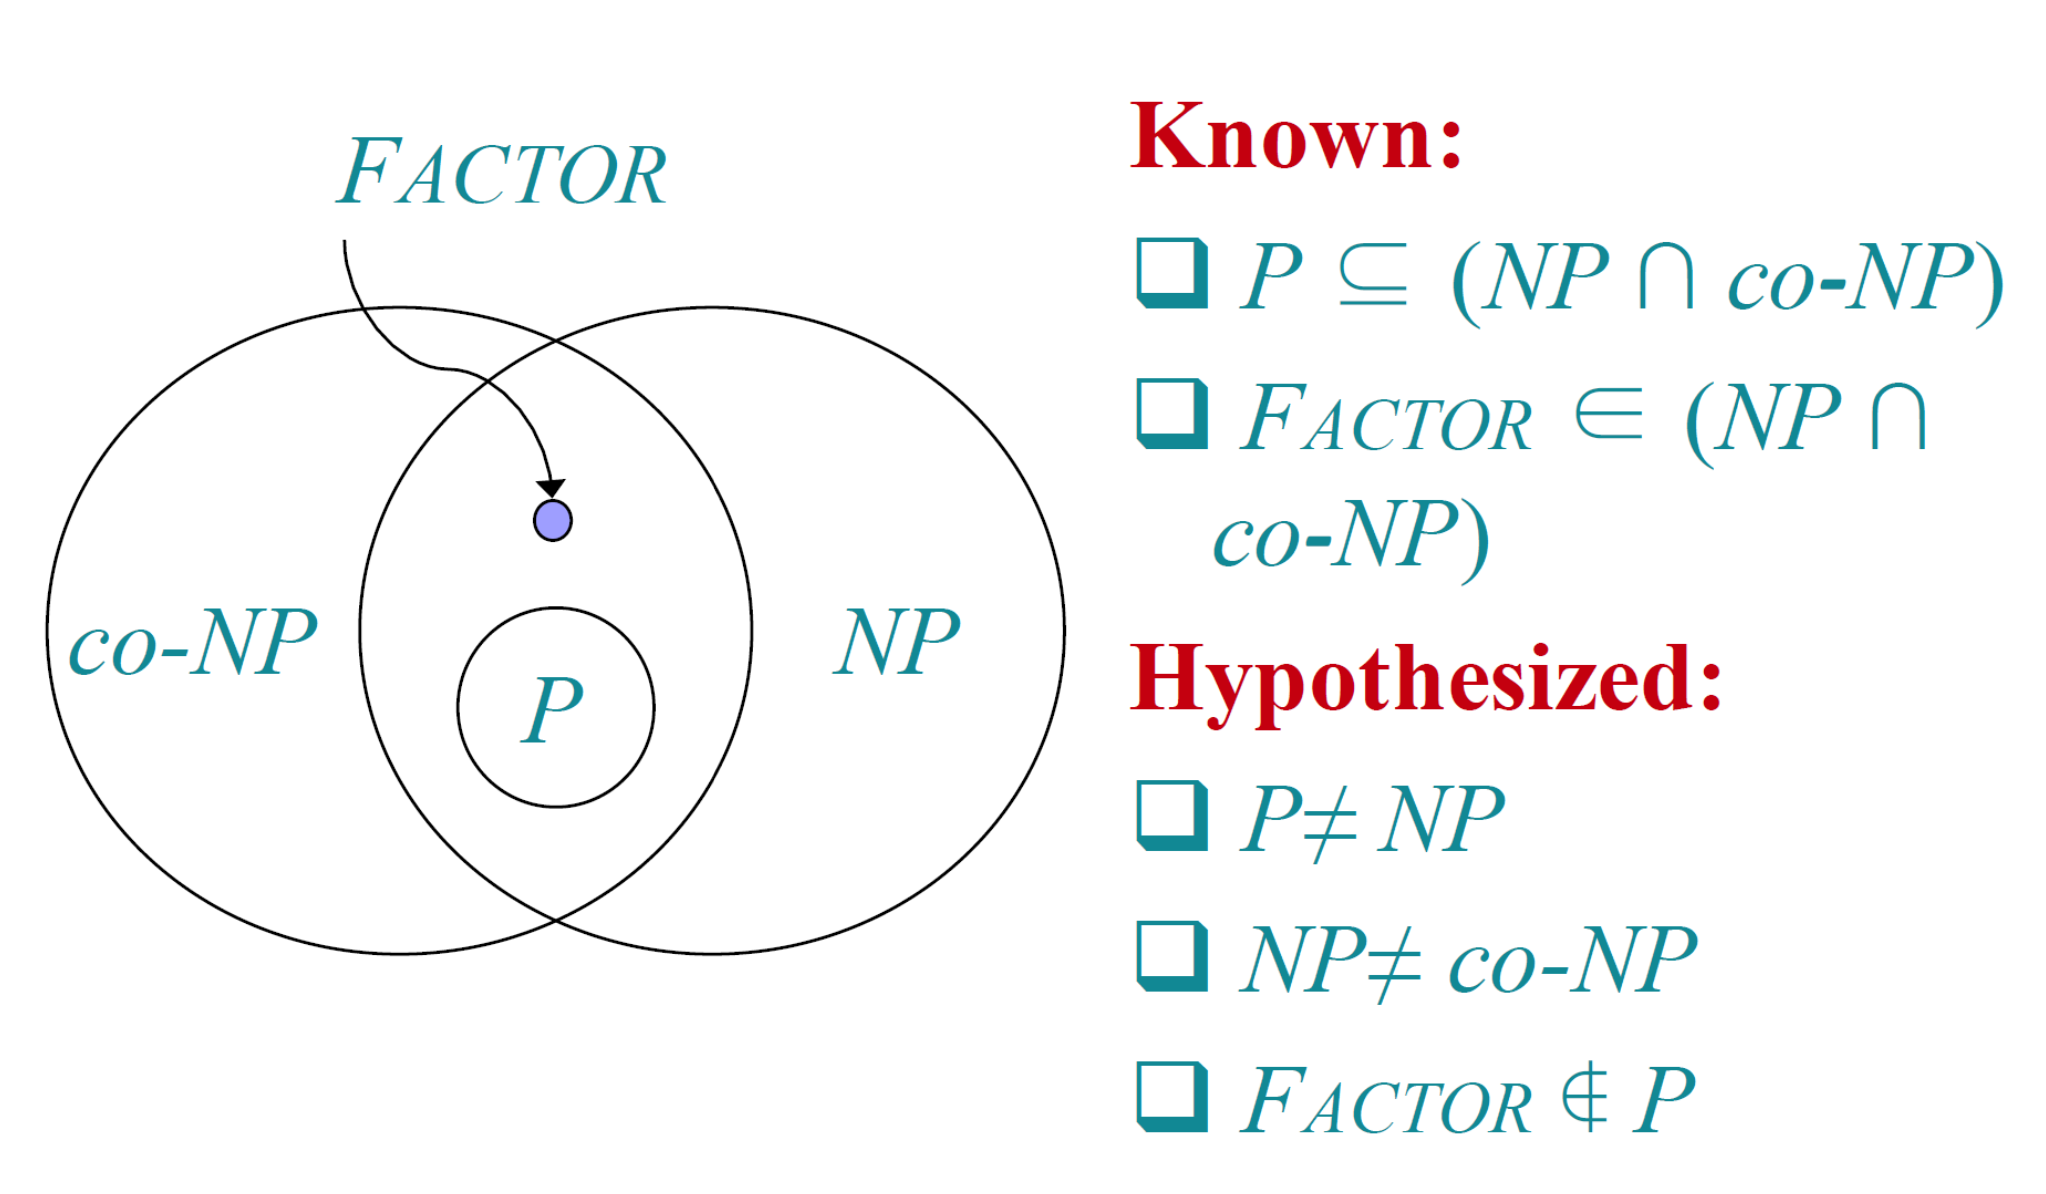
\includegraphics[width=0.8\columnwidth]{L12/likely_relationships}
      \end{center}
\section*{Approximation}
  \subsection*{Minimization / \red{Maximization}} \noindent
    Given an instance, find a solution that has min / \red{max} cost.
    \begin{itemize}[leftmargin=*]
      \item $C^*$ - cost of optimal solution
      \item $C$ - cost of solution found by your algorithm
      \item $\dfrac{C}{C^*}$ / \red{$\dfrac{C}{C^*}$} - approx. ratio, always larger than 1
    \end{itemize}
  \subsection*{PTAS} \noindent
    \subsubsection*{Polynomial-time approximation scheme} \noindent
      An algorithm that given an instance and $\epsilon > 0$, runs in time $poly(n) f(\epsilon)$ for some function $f$, and has approximation ratio $(1 + \epsilon)$
    \subsubsection*{Fully PTAS} \noindent
      An algorithm that given an instance and $\epsilon > 0$, runs in time $poly(n, \frac{1}{\epsilon})$ for some function $f$, and has approximation ratio $(1 + \epsilon)$
\end{multicols*}
\end{document}
